\documentclass[12pt,a4paper,openright,twoside,table]{book}
\usepackage[utf8]{inputenc}
\usepackage{pgfplots}
\usepackage{disi-thesis}
\usepackage{code-lstlistings}
\usepackage{listings}
\usepackage{notes}
\usepackage{shortcuts}
\usepackage{acronym}
\usepackage{float}
\usepackage[normalem]{ulem}
\useunder{\uline}{\ul}{}

% Commands
\newcommand\tab[1][1cm]{\hspace*{#1}}
\newcommand{\imagesource}[5] {
	\begin{figure}[htb]
		\centering
		\includegraphics[width=#4\linewidth]{#1}
		\caption{#3}
		{\scriptsize%
			Source: \url{#2}}
		\label{fig:#5}
	\end{figure}
}

\school{\unibo}
\programme{Corso di Laurea in Ingegneria e Scienze Informatiche}
\title{Pacchettizzazione e Distribuzione Automatizzata di Software JVM-Based}
\author{Marco Sternini}
\date{\today}
\subject{Programmazione ad oggetti}
\supervisor{Dott. Danilo Pianini}
\cosupervisor{Dott.sa Martina Baiardi}
\session{III}
\academicyear{2022-2023}

% Definition of acronyms
\acrodef{vm}[VM]{Virtual Machine}
\acrodef{cicd}[CI/CD]{Continuous Integration Continuous Delivery}
\acrodef{cli}[CLI]{Command Line Interface}
\acrodef{jvm}[JVM]{Java Virtual Machine}
\acrodef{jre}[JRE]{Java Runtime Environment}
\acrodef{aur}[AUR]{Arch User Repository}
\acrodef{dsl}[DSL]{Domain-Specific Language}
\acrodef{kiss}[KISS]{Keep It Simple, Stupid}
\acrodef{dry}[DRY]{Don't Repeat Yourself}
\acrodef{jdk}[JDK]{Java Development Kit}
\acrodef{jit}[JIT]{Just in Time}
\acrodef{aot}[AOT]{Ahead of Time}

\mainlinespacing{1.241} % line spacing in mainmatter, comment to default (1)

\begin{document}

\frontmatter\frontispiece

\begin{abstract}	
Max 2000 characters, strict.
\end{abstract}

\begin{acknowledgements} % this is optional
Optional. Max 1 page.
\end{acknowledgements}

%----------------------------------------------------------------------------------------
\tableofcontents   
\listoffigures     % (optional) comment if empty
\lstlistoflistings % (optional) comment if empty
%----------------------------------------------------------------------------------------

\mainmatter

%!TEX root = ../thesis-main.tex

\chapter{Introduzione}\label{chap:introduction}
Il mondo del software ha scritto diverse decadi di storia. Sin dagli anni '50, quando i primi calcolatori programmabili hanno fatto il loro ingresso sul mercato, il software ha assunto un ruolo sempre più pervasivo nella vita quotidiana delle persone. Oltre ad essere parte integrante dei sistemi informativi delle aziende, lo possiamo trovare anche all'interno di automobili, elettrodomestici e tantissimi strumenti con la quale abbiamo a che fare nella nostra quotidianità. La crescente diffusione del software ha introdotto la necessità di progettare metodologie di sviluppo solide e versatili. Uno dei primi è il \textbf{modello a cascata} il quale struttura il processo di realizzazione del software in fasi sequenziali lineari. Il modello riprende la tipica organizzazione della produzione manifatturiera e fu progressivamente abbandonato con l'evolversi delle richieste del mercato. Successivamente prese piede il concetto di modelli iterativi come il \textbf{modello a spirale} in cui il processo di sviluppo è suddiviso in fasi multiple ripetute più volte (iterazioni). Gli ultimi decenni hanno dato vita a un nuovo modello, considerato lo standard dell'industria, la \textbf{metodologia agile}. Quest'ultima non rappresenta un unico modello, ma un insieme di modelli iterativi costruiti sulla base dei principi definiti all'interno del manifesto agile. Questi principi mettono in primo piano un ambiente autonomo e dinamico in cui sono fondamentali: cicli di sviluppo brevi, continui miglioramenti, la comunicazione col cliente e la consegna tempestiva di funzionalità. Il progetto esposto in questo documento introduce un evoluzione del concetto agile nato recentemente nel mondo dello sviluppo del software, conosciuto come ``DevOps".

\section{Contesto}
Con l'avvento di Internet il concetto di software come un entità sviluppata e finita ha completamente cessato di esistere. Mediante la rete è diventato semplice ed efficiente distribuire un programma e fornire un ulteriore supporto attraverso aggiornamenti evolutivi e correttivi. Il fenomeno è cresciuto tanto da aver dato luce alla pratica del rilascio di applicazioni deliberatamente non complete, le quali attraverso il feedback degli utenti evolvono verso un prodotto finito. Il manifesto agile ha introdotto la cultura di emettere frequenti rilasci di nuove versioni del software, rendendo la distribuzione un punto cardine all'interno del ciclo di vita di esso. Dietro lo sviluppo rapido di nuove funzionalità è necessario il rilascio di queste altrettanto velocemente, la filosofia DevOps nasce per soddisfare questa esigenza.

\subsection{DevOps}
La filosofia DevOps (termine nato dalla contrazione di ``Development" ed ``Operations") si è formata intorno al 2008 con l'idea chiave di unire il team di sviluppo ed il team operativo. Il principale catalizzatore di questo concetto è stata la necessità di affrontare inefficienze nelle fasi del ciclo di vita del software. Differentemente dalla metodologia agile, DevOps è una filosofia di sviluppo software che esprime attraverso tre pilastri il suo obiettivo:

\begin{itemize}
	\item il \textbf{flusso}, il miglioramento del flusso di lavoro lungo l'intero processo di produzione, ciò significa ottimizzare il processo dall'idea, fino alla generazione di valore con il software in produzione.
	\item Il \textbf{feedback}, mediante cicli di feedback rapidi si garantisce la scoperta di difetti nel codice nelle fasi iniziali del ciclo di vita del prodotto. Ciò comporta rapide correzioni, minor debito tecnico e la garanzia di possedere in qualsiasi momento un software stabile e qualitativamente pronto ad un rilascio.
	\item L'\textbf{apprendimento continuo}, la filosofia DevOps promuove la sperimentazione continua, ossia interrogarsi regolarmente sui possibili miglioramenti attuabili assumendosi i rischi che l'applicazione di questi può recare.
\end{itemize}

Le nozioni fornite dalla cultura DevOps ricoprono diversi ambiti e non si limitano agli aspetti tecnici del ciclo di vita del software. Nella pratica esistono diverse tecnologie che concorrono allo sviluppo di processi conformi alla filosofia presentata.

\begin{figure}[htb]
	\centering
	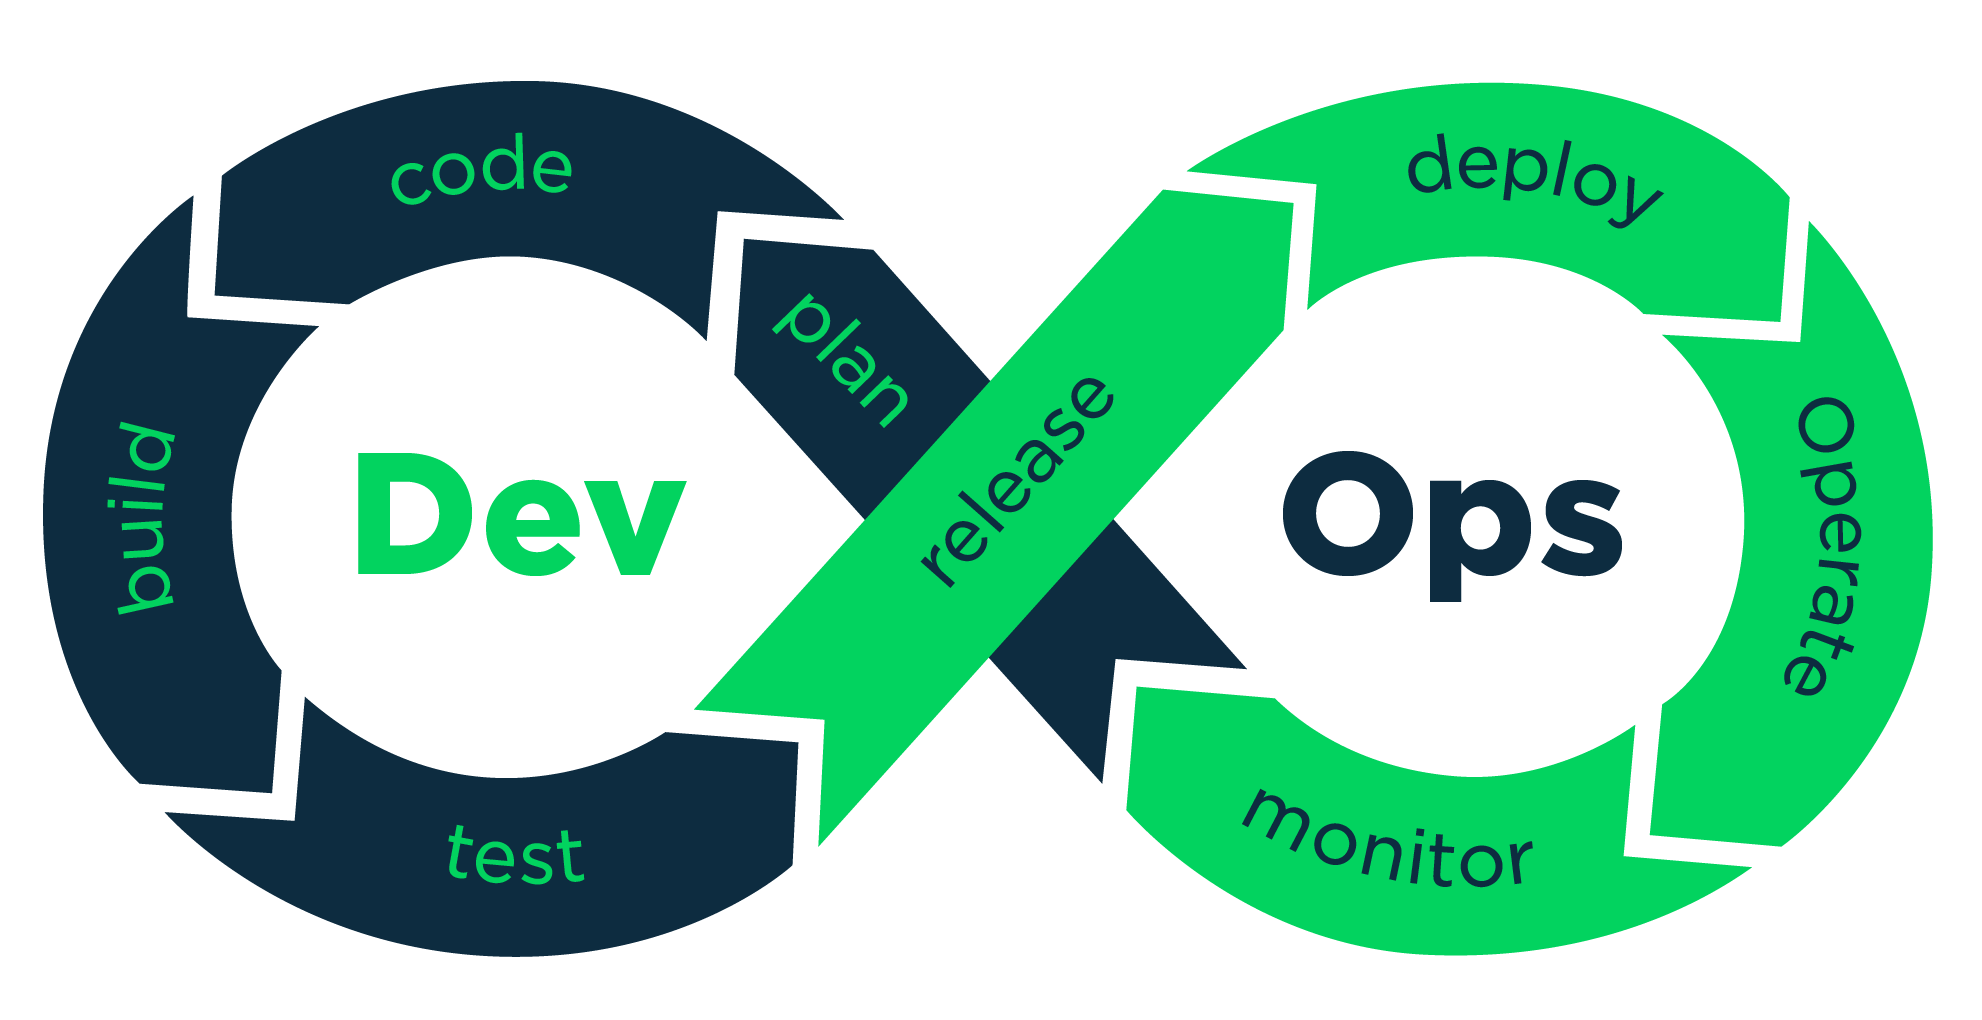
\includegraphics[width=.8\linewidth]{figures/devops-process.png}
	\caption{Le fasi della metodologia DevOps}
	\label{fig:devops-process}
\end{figure}

Il modello illustrato nella figura \ref{fig:devops-process} rappresenta il ciclo di vita del software secondo la filosofia DevOps. La disposizione delle fasi, configurata in modo da evocare il simbolo dell'infinito, simboleggia il concetto di continuità fondamentale per questa filosofia. Questo concetto è introdotto all'interno del flusso mediante un altro pilastro: l'\textit{automazione}. Grazie all'automazione, gli sviluppatori possono delegare compiti complessi o ripetitivi a sistemi esterni configurando tre componenti chiave: un evento, un'azione e il risultato atteso. Quando si verifica un evento specifico, un'entità esterna esegue un insieme di azioni predeterminate, il cui successo o fallimento viene determinato dal confronto con il risultato atteso. A livello pratico, ciò è ottenuto mediante l'utilizzo di server o più generalmente infrastrutture cloud complesse.

L'automazione dunque garantisce l'esecuzione dei processi in modo consistente e permette di concentrare le risorse del team sullo sviluppo, eliminando quindi l'intervento umano da compiti ripetitivi e passibili di errori. Una delle pratiche più diffuse, concetto rilevante della filosofia DevOps, è la pipeline di \ac{cicd}.

\paragraph{Continuous integration} La pratica della \textit{continuous integration} si concentra sull'integrazione automatica e continua delle modifiche al codice sorgente del progetto. Tipicamente, il processo si articola nei seguenti passaggi: (i) gli sviluppatori introducono nuovo codice nel progetto attraverso il software di \textit{version control}, (ii) un server acquisisce le modifiche, compila e testa l'intero progetto, (iii) una volta completato il processo, comunica agli sviluppatori l'esito delle operazioni. Questo approccio consente di individuare errori nel codice anticipatamente, garantendo stabilità e una maggiore qualità al software.

Un aspetto fondamentale è la stesura dei test: un'eccessiva copertura può rallentare il processo di integrazione. È pertanto essenziale bilanciare la copertura dei test in base alle esigenze del progetto, tenendo presente che un aumento della copertura riduce il rischio di introdurre codice difettoso.

\paragraph{Continuous delivery} La distribuzione rappresenta l'insieme di operazioni finalizzate alla consegna del software agli utenti finali. Questo processo estende l'integrazione continua e si preoccupa di garantire la disponibilità costante di un artefatto di build pronto per il rilascio. L'effettivo rilascio di una nuova versione del software può avvenire in modo automatico oppure manualmente da parte dello sviluppatore. La filosofia DevOps fornisce linee guida e non regole rigide, lasciando al team di sviluppo il compito di progettare ed integrare un flusso adeguato alle necessità del progetto.

\subsection{Software JVM-based}
Per "software \ac{jvm}-based" si intendono i programmi e le applicazioni realizzate mediante linguaggi di programmazione eseguiti e compilati per la \ac{jvm}. Nata nel 1995, la Java Virtual Machine ha rivoluzionato il mondo dello sviluppo del software introducendo un nuovo livello di astrazione nella compilazione ed esecuzione dei programmi. Il linguaggio Java, sviluppato appositamente per l'omonima macchina virtuale, è un linguaggio di programmazione ad alto livello orientato agli oggetti progettato per avere il minor numero di dipendenze esterne possibile, in modo da garantire la sua portabilità. L'esecuzione di un programma Java avviene per fasi differenti rispetto ad un normale linguaggio compilato: il codice viene tradotto, in una prima fase di compilazione, in \textit{bytecode}, un linguaggio intermedio. Quest'ultimo è successivamente fornito alla macchina virtuale, la quale interpreta il bytecode generato ed esegue quindi il programma.

Inizialmente progettata per ospitare il linguaggio Java, nel corso del tempo la \ac{jvm} ha visto l'adozione di diversi altri linguaggi di programmazione e l'adattamento di alcuni provenienti da ambienti diversi. Il suo impatto nel mondo del software fu ed è ancora attualmente rilevante, tanto che due indici di valutazione della popolarità dei linguaggi di programmazione posizionano i due principali linguaggi \ac{jvm} all'interno della top 20, con Java, il più datato, nella top 5 (TIOBE\footnote{https://www.tiobe.com/tiobe-index/} e PYPL\footnote{https://pypl.github.io/PYPL.html} index). Una delle caratteristiche che ha decretato il successo di questa architettura è la portabilità. L'integrazione di un linguaggio intermedio permette di astrarre dalla piattaforma di esecuzione, consentendo, mediante un singolo codice sorgente, di distribuire l'applicativo su differenti sistemi operativi con persino architetture hardware diverse.

% Nella figura \ref{fig} è illustrato

Un aspetto cruciale nel rilascio di un'applicazione è la sua distribuzione. La forma e il metodo adottati devono garantire un processo di installazione scorrevole, privo di intoppi e consistente, in modo che gli utenti possano installare l'applicativo nel proprio sistema senza preoccuparsi di dipendenze esterne. Tuttavia, questa necessità presenta sfide specifiche nell'ambito dei linguaggi di programmazione interpretati, come quelli \ac{jvm}-based.

\subsection{Problemi della pacchettizzazione nei software JVM}
L'esecuzione di un programma Java richiede inevitabilmente la presenza di una \ac{jvm}, o più precisamente un \ac{jre}, ossia un ambiente di esecuzione opportuno. Generalmente i software sono distribuiti mediante due tipologie di archivi differenti.

\section{Obiettivi}
I punti discussi precedentemente hanno evidenziato l'importanza che l'automazione ricopre all'interno dello sviluppo del software. Il rilascio continuo di un applicazione è necessario per mantenere elevati standard di qualità e comporta la necessità di automatizzare questi processi per garantire la loro esecuzione in modo consistente. Inoltre, la distribuzione dell'applicativo deve avvenire mediante mezzi compatibili e diffusi per assicurare un processo di installazione semplice e funzionale agli utenti. Il package management system in questo ambito offre un approccio valido: le diverse distribuzioni Linux adoperano esso dagli albori e nei restanti due sistemi operativi, Windows e MacOs, il suo utilizzo si sta diffondendo sempre maggiormente.
\begin{figure}[htb]
	\centering
	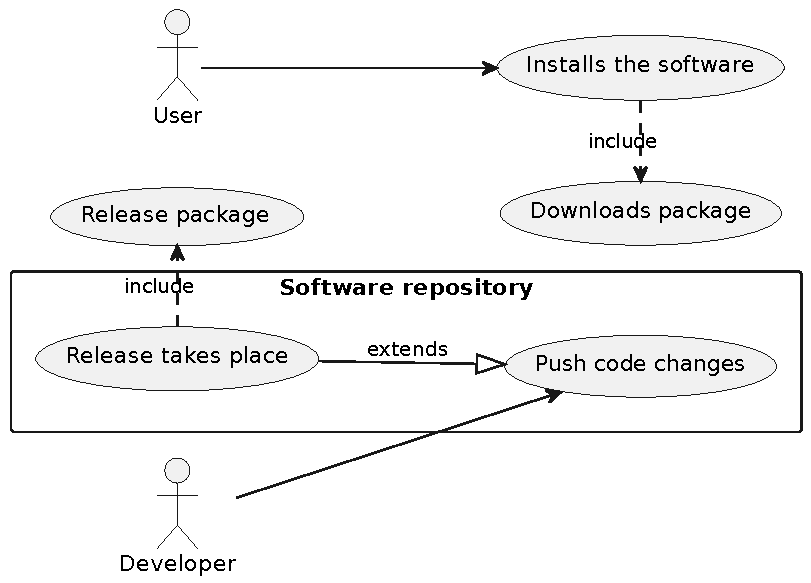
\includegraphics[width=.75\linewidth]{figures/use-case-diagram.pdf}
	\caption{Diagramma dei casi d'uso dallo sviluppatore all'utente}
	\label{fig:use-case-diagram}
\end{figure}

L'obiettivo principale dell'elaborato è quindi quello di progettare un sistema di pacchettizzazione e distribuzione del software automatico all'interno di una pipeline di integrazione e distribuzione continua. I nuovi processi devono integrarsi all'interno dell'attuale pipeline di Alchemist, estendendo le funzionalità di assemblaggio e rilascio del software. La distribuzione del pacchetto software deve avvenire per mezzo di repository pubblici diffusi, in modo da raggiungere il numero maggiore possibile di utenti; essa, inoltre, deve avvenire consistentemente nell'istante in cui una nuova versione di Alchemist viene rilasciata. La totalità dei processi integrati, inoltre, deve prevedere l'esecuzione di test all'interno del flusso, in modo da fornire un riscontro immediato nell'eventualità gli artefatti siano difettosi. Nella \Cref{fig:use-case-diagram} sono rappresentati gli scenari di utilizzo da parte degli utenti finali e degli sviluppatori di Alchemist. In particolare, lo sviluppatore introduce nuovo codice all'interno del repository del progetto e successivamente l'esecuzione della pipeline determina se è necessario il rilascio di una nuova versione. In caso di esito positivo, vengono generati i pacchetti software di installazione. Questi pacchetti, una volta distribuiti, consentiranno agli utenti di introdurre Alchemist nel proprio sistema.
%!TEXroot = ../thesis-main.tex

\chapter{Scenario di riferimento}\label{chap:scenery}

L'introduzione ha delineato gli obiettivi e le motivazioni che guidano il progetto, evidenziando il valore aggiunto che esso porta nell'ambito della distribuzione del software. Nel capitolo seguente, verrà presentato il software di riferimento oggetto dell'elaborato.

\section{Un software complesso}\label{sec:alchemist}
Il software selezionato per questo progetto è stato scelto in base a criteri fondamentali. In primo luogo, la sua complessità, in quanto garantisce che sia stato sviluppato in modo robusto e con elevati standard di qualità. In secondo luogo, la presenza di una solida infrastruttura di \ac{cicd}, poiché permette di focalizzare il progetto sulla pacchettizzazione e la presenza di un flusso ben testato pone le basi per integrare i processi di distribuzione richiesti. Il terzo requisito richiede che l'applicativo sia stato sviluppato specificamente per essere eseguito su una \ac{jvm}, al fine di esplorare le diverse metodologie di pacchettizzazione confrontandosi con i problemi che il processo comporta per questa specifica tipologia di programmi.

\subsection{Alchemist}

Un software che soddisfa ampiamente le richieste è Alchemist\cite{Pianini_2013}, un framework di simulazione stocastico open-source sviluppato dall'Università di Bologna, progettato per modellare elementi di programmazione pervasiva. Quest'ultima si riferisce a un paradigma in cui la computazione è integrata ovunque in modo onnipresente e invisibile (\textit{ubiquitous computing}). 

\imagesource{figures/alchemist-metamodel.pdf}{https://alchemistsimulator.github.io/explanation/metamodel/}{Il meta-modello di Alchemist}{.9}{alchemist-metamodel}

Il software si presenta come un simulatore, perciò per comprendere il suo utilizzo è necessario introdurre il concetto di simulazione in ambito scientifico. Per simulazione si intende un modello della realtà, costruito secondo le regole di un analista, sviluppato per consentire la valutazione dello svolgersi di una serie di eventi in un ambiente definito. Mediante la definizione delle entità e le regole che coinvolgono il modello studiato, l'analista attraverso Alchemist crea e osserva simulazioni atte a modellare interazioni tra agenti autonomi in ambienti dinamici: ossia scenari di \textit{aggregate} e \textit{nature-inspired computing}. Il meta-modello di Alchemist descrive gli elementi e le relazioni con cui l'utente finale è capace di costruire simulazioni di scenari complessi; come si può notare dalla \cref{fig:alchemist-metamodel}, le entità in gioco sono ispirate ai fondamenti della chimica. 

\paragraph{Architettura} Un aspetto importante per lo svolgimento del progetto è l'architettura del software in oggetto, la quale deve soddisfare i requisiti posti inizialmente. In questo contesto il framework propone una struttura consona, in quanto è realizzato mediante linguaggi JVM-based, più precisamente Java e Kotlin, e utilizza un'architettura modulare ed estendibile, sinonimo di robustezza. 

Il simulatore, come già citato, è un progetto open-source, ossia distribuito sotto termini di una licenza aperta. Questa permette a chiunque di osservare il codice sorgente e di contribuire allo sviluppo del progetto, coordinato da un personale responsabile del suo avanzamento. La natura open-source del progetto apre le porte a modalità di sviluppo del codice differenti rispetto a team predefiniti di dimensioni ridotte; in un progetto aperto, gli utenti che contribuiscono allo sviluppo sono potenzialmente infiniti, ragion per cui l'automazione risulta determinante per mantenere un processo ordinato e controllato di integrazione e rilascio del software. Alchemist, in quest'ottica, presenta un'infrastruttura di \ac{cicd} solida, nello specifico integra:
\begin{enumerate}
	\item il test e l'analisi statica del codice;
	\item la costruzione automatica di artefatti come la documentazione;
	\item il versioning automatico del software a ogni rilascio;
	\item la pubblicazione, mediante le release GitHub, degli archivi JAR dell'applicazione.
\end{enumerate}
L'insieme di queste azioni (a eccezione del rilascio, il quale avviene sotto certe condizioni) è eseguito in modo continuo ogni qualvolta del codice è introdotto nel repository: tramite una pull request esterna o attraverso una modifica diretta svolta dal maintainer del progetto.

\paragraph{Modalità di utilizzo} Il simulatore offre due modalità di utilizzo concepite per soddisfare esigenze diverse. 
Come chiaramente illustrato nella documentazione\footnote{https://alchemistsimulator.github.io/howtos/preparation/jar/index.html}, la modalità di utilizzo consigliata coinvolge l'impiego di Gradle. Quest'ultimo consente all'utente, generalmente un programmatore o un utente con competenze avanzate, di sfruttare Alchemist al massimo delle sue potenzialità; tale approccio risulta quindi più indicato quando è necessario avere un controllo completo per sviluppare simulazioni complesse. Il secondo approccio coinvolge l'utilizzo della \ac{cli} per avviare e osservare una simulazione di Alchemist. Mediante l'interfaccia a linea di comando si fornisce al simulatore un file descrittivo che elenca le entità e le regole della simulazione utilizzando gli elementi descritti nel meta-modello. Successivamente l'applicazione avvia l'esecuzione e l'utente può, secondo modalità scelte da lui stesso, osservare graficamente l'evolversi della simulazione.

L'obiettivo dell'elaborato è migliorare il processo di installazione e di onboarding del software, focalizzandosi in particolare sulla seconda modalità di utilizzo. Per fare ciò, si prevede di distribuire pacchetti di installazione \textit{self-contained}, eliminando così la dipendenza da risorse esterne che gli archivi JAR comportano. Inoltre, si intende fornire il supporto ai package manager, al fine di semplificare ulteriormente il processo di download e aggiornamento del software per gli utenti.

\section{Tecnologie}\label{sec:technologies}

Alchemist utilizza diversi strumenti per sviluppare la sua infrastruttura di \ac{cicd}. Nella seguente sezione sono esposti i principali, i quali sono protagonisti del progetto esposto in questo elaborato.

\subsection{Gradle}

Mentre in passato la produzione di artefatti (documentazione, pacchetti, eseguibili) era delegata a script costruiti dallo sviluppatore, in un progetto di grandi dimensioni è oggigiorno essenziale avvalersi di uno strumento di \textit{build automation}. Come l'output di un programma deterministico non cambia per uno stesso input, la produzione di artefatti deve essere consistente e riproducibile riducendo al minimo l'intervento umano. 

Gradle\footnote{https://gradle.org/} è uno dei tanti strumenti disponibili, supporta diversi linguaggi di programmazione, anche se risulta popolare nell'ambiente JVM come alternativa a Maven. I \textit{task} sono l'unità minima di esecuzione e rappresentano un azione: come generare un JAR, eseguire dei test o produrre la documentazione. Mediante direttive come \textit{dependsOn} è possibile creare dipendenze tra processi: Gradle orchestra l'esecuzione dei task costruendo un grafo aciclico diretto (DAG) delle dipendenze. L'esecuzione di Gradle (\cref{fig:gradle-build-lifecycle}) avviene in tre fasi distinte elencate di seguito:

\imagesource{figures/gradle-build-lifecycle-example.png}{https://docs.gradle.org/current/userguide/build_lifecycle.html}{Esempio di inizializzazione, configurazione ed esecuzione di una build Gradle}{1}{gradle-build-lifecycle}

\begin{enumerate}
	\item \textbf{Fase di inizializzazione}: in primo luogo Gradle crea un'istanza di Settings che organizza l'architettura del progetto. Attraverso un file, di nome ``settings.gradle", lo sviluppatore stabilisce il progetto radice e tutti gli eventuali progetti figli. 
	\item \textbf{Fase di configurazione}: successivamente tutti i file di configurazione ``build\-.\-gradle" (del progetto radice e tutti i sotto-progetti) vengono analizzati per costruire il grafo dei task.
	\item \textbf{Fase di esecuzione}: infine, Gradle esegue i task richiesti considerando le dipendenze descritte nel grafo generato nella fase precedente.
\end{enumerate}

Un componente chiave sono i plugin, i quali consentono di estendere le funzionalità di Gradle: aggiungere nuovi task, estendere il modello con nuovi elementi e applicare configurazioni specifiche all'intero progetto. La presenza di diversi plugin base e altri creati dalla comunità rende Gradle uno strumento molto versatile. Nel progetto Alchemist, Gradle è utilizzato in modo esteso e costituisce il build system del software, si occupa inoltre di gestire le dipendenze, costruire gli artefatti ed eseguire gli unit test.

\subsection{GitHub Actions}

Tramite Gradle lo sviluppatore è in grado di eseguire procedure articolate come compilazione, test e dispiegamento utilizzando un semplice comando da \ac{cli}. L'invocazione di queste procedure richiede però l'intervento umano, è quindi necessario uno strumento capace di automatizzare i processi offrendo un infrastruttura resiliente e facilmente accessibile.

GitHub Actions è una piattaforma di \ac{cicd} disponibile per i repository ospitati su GitHub, che consente la configurazione ed esecuzione di pipeline personalizzate, chiamate \textit{workflow}. Questi \textit{workflow} sono flussi di processi che consistono in un insieme di \textit{job} eseguiti sequenzialmente o parallelamente all'interno di macchine virtuali denominate \textit{runner}. I workflow (\cref{fig:github-actions-example}) sono descritti in file YAML all'interno di una cartella specifica del repository. Questi file definiscono i passaggi (\textit{step}) e le azioni (\textit{action}) che il runner deve eseguire all'interno di \textit{job}, macro-processi incaricati all'esecuzione sequenziale di step.

\imagesource{figures/overview-actions-simple.png}{https://docs.github.com/en/actions/learn-github-actions/understanding-github-actions}{Sintesi dei componenti utilizzati su GitHub Actions ed esempio di un workflow}{.8}{github-actions-example}

Uno step rappresenta l'unità minima di esecuzione all'interno della piattaforma Actions. Le API supportano due differenti tipologie di step: (i) le azioni, ossia componenti riutilizzabili e parametrizzabili delegati all'esecuzione di una procedura specifica e (ii) i comandi shell o script. Le azioni possono essere create personalmente o riutilizzate attingendo da un vasto marketplace manutenuto dalla comunità. Per esempio, una delle azioni più diffuse è ``actions/checkout" [\cite{github-actions-diffusion}], la quale clona il repository del progetto nella cartella di lavoro corrente del runner.

%!TEX root = ../thesis-main.tex

\chapter{Analisi}

\section{Requisiti}

Il progetto si pone due principali obiettivi:
\begin{itemize}
	\item La generazione automatica di pacchetti di installazione multi-piattaforma.
	\item La pubblicazione automatica dei rilasci del software all'interno di repository pubblici selezionati.
\end{itemize}
Un pacchetto software è un insieme di risorse necessarie per eseguire un'applicazione o un servizio su un sistema. Sono usualmente distribuiti all'interno di archivi compressi contenenti meta-dati che ne descrivono la forma e l'utilizzo. La pubblicazione è l'atto di inserire il software in archivi (repository) online con l'intento di consentire l'installazione agli utenti finali. Entrambi i processi devono essere automatizzati e integrati all'interno di una pipeline di integrazione e rilascio continua.

\paragraph{Requisiti funzionali}

Le funzionalità richieste si possono classificare in due gruppi distinti: il primo contiene tutto ciò che concerne l'esperienza dell'utente finale, mentre il secondo descrive le funzionalità dal punto di vista degli sviluppatori e contributori di Alchemist. Di seguito il primo gruppo:
\begin{itemize}
	\item \textbf{Pacchettizzazione}: il simulatore deve essere distribuito in pacchetti \textit{self-contained}, ossia contenenti l'intera applicazione, e più specificatamente nell'ambito \ac{jvm}, integranti un \ac{jre} adibito all'esecuzione.
	\item \textbf{Multi-piattaforma}: Alchemist deve essere installabile sui maggiori sistemi operativi in circolazione come Windows, MacOS e le principali distribuzioni Linux.
	\item \textbf{Plug and play}: l'installazione non deve richiedere configurazioni complesse, l'applicativo deve essere pronto all'uso non appena installato.
\end{itemize}

I requisiti del gruppo successivo sono accumunabili per il loro scopo, vale a dire l'automazione:

\begin{itemize}
	\item \textbf{Automazione dei pacchetti}: la generazione dei pacchetti di installazione deve essere automatica e configurabile.
	\item \textbf{Automazione della distribuzione}: il rilascio di una nuova versione comprende la distribuzione di essa nei repository selezionati e deve essere svolta in modo automatico.
	\item \textbf{Verifica funzionamento}: entrambi i processi descritti precedentemente devono essere corredati da verifiche del loro funzionamento e devono bloccare la procedura di rilascio nell'eventualità siano presenti errori.
\end{itemize}

\paragraph{Requisiti non funzionali}

\begin{itemize}
	\item Trattandosi Alchemist di un software in continuo sviluppo, è auspicabile l'utilizzo degli strumenti già impiegati nel progetto. \\ L'integrazione di nuovi applicativi deve essere eseguita solo se strettamente necessaria.
	\item La pipeline \ac{cicd} ottenuta deve garantire prestazioni in linea con la versione precedente l'intervento di questo progetto.
\end{itemize}

\section{Pacchettizzazione}\label{sec:packaging}

Come si evince dall'analisi svolta, la pacchettizzazione è un requisito fondamentale dell'elaborato. Sino a ora l'applicativo Alchemist era distribuito in file JAR, ossia archivi java compressi contenenti tutte le dipendenze e i relativi \textit{classfiles} necessari all'esecuzione. Quest'approccio molto diffuso porta con sè diverse limitazioni tra cui:
\begin{itemize}
	\item la necessità dell'utente scaricante di avere un \ac{jre} installato nel proprio dispositivo;
	\item il potenziale bisogno di utilizzare un ambiente \ac{jre} specifico e quindi per l'utente di non possedere una versione dell'ambiente compatibile;
	\item la difficoltà di utilizzo per utenti non esperti, abituati a eseguire programmi utilizzando file eseguibili nativi della propria piattaforma.
\end{itemize}
Alcune di queste restrizioni risultano mitigate, tuttavia non in tutte le piattaforme, come Windows, il quale per esempio non fornisce un ambiente java pre-installato. Esistono diversi strumenti di terze parti e non che cercano di far fronte a questo problema, è importante dunque valutare e scegliere lo strumento più opportuno.

\subsection{Soluzioni}

Nell'ottica di semplificare la configurazione di questo processo lo strumento selezionato deve supportare le tre principali piattaforme descritte nei requisiti precedentemente. Tra gli strumenti analizzati due molto differenti si sono distinti, vale a dire: \textit{jpackage}, comando disponibile nel \ac{jdk} dalla versione 14, adibito alla produzione di pacchetti self-contained con \ac{jre} integrata e \textit{GraalVM}, un \ac{jdk} sviluppato da Oracle che fornisce un compilatore \ac{jit} e \ac{aot} per java. 

La modalità \ac{jit} descrive il comportamento normale di ogni \ac{jvm}: il compilatore Java traduce il programma ad alto livello in bytecode, e successivamente la \ac{jvm} converte dinamicamente il bytecode in linguaggio macchina per l'architettura specifica. In contrasto la tecnica \ac{aot} ricorda i linguaggi di programmazione compilati, ovvero la compilazione è statica e avviene prima dell'esecuzione del programma. Il compilatore \ac{aot} chiamato ``Native Image", consente di compilare un programma java (e altri linguaggi di programmazione) ottenendo in output un eseguibile nativo per ogni piattaforma. Quest'ultimo inoltre porta con sè diversi vantaggi come: un minor costo in risorse CPU e memoria, tempi di avvio minori e dimensioni ridotte rispetto un normale programma java distribuito con un \ac{jre}. La compilazione \ac{aot} però ha dei requisiti, uno di questi fondamentale è la \textit{closed world assumption}: ossia ogni parte di codice raggiungibile in esecuzione lo deve essere anche in fase di build. Ciò accade perché native image svolge un analisi statica del codice, pertanto alcune funzionalità come la reflection oppure il caricamento dinamico non sono supportate e richiedono una soluzione alternativa.

In contrasto \textit{jpackage} fornisce uno strumento interessante, il quale non richiede modifiche all'applicativo ed è pre-installato in tutti i \ac{jdk} dalla versione 14 e successive. Lo strumento risolve le problematiche esposte inizialmente mediante l'annessione di un \ac{jre} utilizzando \textit{jlink}. Inoltre, produce diverse tipologie di pacchetti per ogni piattaforma ed è completamente controllabile da interfaccia \ac{cli}. Le tipologie di pacchetti generabili sono elencate di seguito:
\begin{itemize}
	\item \textit{exe} e \textit{msi} per Windows;
	\item \textit{rpm} e \textit{deb} per Linux;
	\item \textit{pkg} e \textit{dmg} per MacOs.
\end{itemize}
Tuttavia anch'esso presenta dei limiti come: la necessità di essere eseguito sullo stesso sistema operativo dove i pacchetti prodotti sono destinati (lo stesso vale per GraalVM, la \textit{cross compilation} non è supportata) e la produzione di un solo pacchetto per singola esecuzione.

\paragraph{Valutazione finale} Ambedue le soluzioni, seppure differenti concorrono all'obiettivo primario: la distribuzione del software multi-piattaforma. GraalVM fornisce diversi vantaggi prestazionali, ma i requisiti da esso richiesti non sono compatibili con l'architettura del simulatore. D'altro canto jpackage fornisce tutto il necessario per costruire i pacchetti con embed di un \ac{jre} senza la necessità di stravolgere l'architettura del software, e i limiti delineati sono superabili adoperando script o configurazioni specifiche.

\section{Analisi degli strumenti}

Gli strumenti presentati nella sezione \ref{sec:technologies} costituiscono il progetto Alchemist nel suo complesso. Grazie agli script Gradle, il simulatore gestisce in modo efficace i processi di compilazione, generazione della documentazione ed esecuzione delle verifiche del codice. Mentre l'utilizzo della piattaforma Actions fornisce l'infrastruttura necessaria e le API per creare una pipeline di \ac{cicd}. 

\begin{figure}[htb]
	\centering
	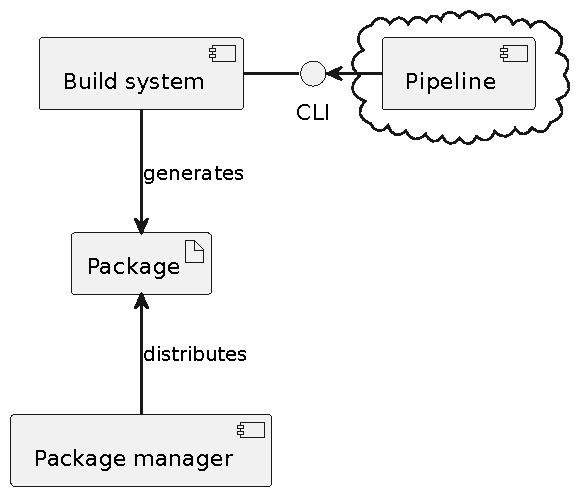
\includegraphics[width=.6\linewidth]{figures/components-diagram.pdf}
	\caption{Diagramma dei componenti che interagiscono nel progetto}
	\label{fig:components-diagram}
\end{figure}

In considerazione dei requisiti posti, la pacchettizzazione risulta un processo di produzione di artefatti ed è perciò necessaria la sua integrazione nel build system. Mediante l'integrazione, si garantisce un corretto ordine di esecuzione rispetto ai diversi processi che il simulatore configura, con l'effetto di minimizzare l'incidenza di errori e assicurando la produzione di pacchetti conformi su qualsiasi sistema operativo in cui Gradle viene eseguito. Contemporaneamente Actions si occupa di offrire l'infrastruttura per automatizzare i processi esposti dal build system. La piattaforma fornisce le funzionalità necessarie a soddisfare i requisiti di automazione posti precedentemente, in particolare mediante: la possibilità di utilizzare macchine virtuali (runner) di tutte e tre i sistemi operativi target, la possibilità di configurare eventi o esecuzioni ricorrenti di processi e tramite la presenza di un'infrastruttura cloud resiliente per l'esecuzione della pipeline. Nel diagramma rappresentato nella \cref{fig:components-diagram}, sono illustrate le interazioni tra gli strumenti descritti. La pipeline, eseguita in un ambiente cloud, utilizza l'interfaccia fornita dal build system per generare il pacchetto di installazione e distribuirlo in modo che sia accessibile tramite i gestori di pacchetti designati.

\subsection{Distribuzione dei pacchetti}

La distribuzione ricopre un ruolo centrale nel processo di rilascio del software. L'obiettivo principale è estendere la disponibilità del simulatore Alchemist attraverso il maggior numero possibile di repository, al fine di permettere a più utenti possibili di installare e utilizzare il software. Nei prossimi paragrafi, verranno presentate due principali piattaforme di distribuzione coinvolte in questo progetto

\paragraph{Arch User Repository} Tra i numerosi fork Linux, Arch occupa una posizione di rilievo nel panorama. Basata sull'architettura x86-64, Arch Linux è stata sviluppata con l'adesione alla filosofia \ac{kiss}. Conosciuta per la sua leggerezza, velocità, e la sua estrema scalabilità, questa distribuzione si distingue per la sua capacità di adattarsi alle esigenze specifiche di ogni utente. Data la sua natura minimalista, l'installazione iniziale non incorpora alcun strumento di configurazione automatica, nessun ambiente desktop e nessun altro strumento necessario all'avvio del sistema. 

Il sistema di gestione dei pacchetti si chiama \textit{pacman} e a differenza dei concorrenti, opera sia a basso che ad alto livello. Un pacchetto non è altro che un file shell script, denominato \textit{PKGBUILD}, contenente le istruzioni necessarie a scaricare i sorgenti e compilarli attraverso un comando: \textit{makepkg}. La linearità dei file PKGBUILD rende la creazione di pacchetti alla portata di qualsiasi utente, difatti Arch supporta l'\textbf{\ac{aur}}, un tratto distintivo di questa distribuzione. Si tratta di un repository di pacchetti in cui qualsiasi utente, anche non sviluppatore, può contribuire. Pertanto, la facilità di accesso e la mancanza di requisiti stringenti danno luce a un ambiente perfetto per la distribuzione del simulatore.

\paragraph{Windows e winget} Un discorso differente vale per Windows, dove fino a poco tempo fa non era previsto alcun package manager ufficiale pre-installato. Gli utenti solitamente installavano software attraverso pacchetti distribuiti in siti web ad-hoc, store non ufficiali o tramite il Microsoft Store. D'altra parte gli sviluppatori, per sfruttare i benefici della gestione a pacchetti, ricorrono a gestori di terze parti. Solamente nel settembre 2020 è stato introdotto ``winget": un package-management system open-source sviluppato da Microsoft, che supporta pacchetti di installazione EXE, MSIX e MSI. Il repository dei pacchetti è accessibile pubblicamente ed è possibile mediante richieste di contribuzione e previa approvazione, pubblicare pacchetti all'interno di esso. \\

Poiché Windows e MacOs sono sistemi operativi closed-source, essi non richiedono particolari attenzioni in quanto le tipologie di pacchetti generabili da jpackage sono sufficienti e ufficialmente supportate. Linux al contrario è notevolmente frammentato, ogni distribuzione può adottare uno dei tanti sistemi di gestione dei pacchetti o introdurne uno nuovo. Purtroppo, non esistono statistiche ufficiali riguardo la diffusione delle distribuzioni, molte di esse si basano su stime o dati non attendibili. D'altra parte, analizzando i pacchetti generabili da jpackage possiamo trarre delle conclusioni.
\begin{itemize}
	\item \textbf{RPM} significa "RedHat Package Manager" ed è un formato di pacchetti progettato per RedHat e le distribuzioni derivate. 
	\item \textbf{DEB} è l'abbreviazione di ``Debian packages", è una tipologia di pacchetto supportata da Debian e le distribuzioni derivate. Secondo distrowatch\footnote{https://distrowatch.com/}, Debian Linux presenta più di 400 distribuzioni derivate e più di 120 di queste sono attualmente attive.
\end{itemize}
È evidente come le due tipologie coprano un ampio spettro nel panorama Linux. Inoltre, esse sono supportate dallo script PKGBUILD nativamente, poiché il comando \textit{makepkg} supporta l'estrazione di questi pacchetti in modo autonomo. 

In conclusione, jpackage fornisce tutto il necessario per supportare in modo completo le piattaforme closed-source disponibili. Riguardo a Linux, i due tipi di pacchetti descritti svolgono un ruolo fondamentale nell'integrare diverse distribuzioni e rendere il software compatibile con l'\ac{aur}, contribuendo così ad ampliare la sua compatibilità nel vasto panorama delle distribuzioni Linux.

%!TEX root = ../thesis-main.tex

\chapter{Design}
Alchemist, come esplicato nella sezione \ref{sec:alchemist}, è un software modulare complesso in continuo sviluppo, le tecnologie illustrate trovano già impiego nel progetto, ad eccezione del software di impacchettamento il quale è oggetto di questo elaborato. Di seguito sarà illustrata l'architettura e l'interazione tra i componenti principali che compaiono nel processo di automazione.

\section{Architettura e macrostruttura}
L'analisi del progetto espone il coinvolgimento di tre diversi componenti per conseguire gli obiettivi di automazione e distribuzione del software. I tre componenti sono definiti come segue: 
\begin{itemize}
	\item \textbf{Build system}: l'insieme dei processi e delle funzioni adibite alla produzione di artefatti. In particolare questo componente richiede lo sviluppo di nuovi processi destinati alla produzione dei pacchetti, test di quest'ultimi e costruzione dei metadati necessari alla distribuzione del software.
	\item \textbf{Pipeline}: il processo automatizzato adibito alla gestione del flusso di lavoro del software, dalla compilazione al rilascio. Questo componente è già impiegato all'interno del progetto Alchemist per gestire l'attuale processo di integrazione continua, il design discusso in questo capitolo inserisce nuovi step all'interno del processo.
	\item \textbf{Release}: l'insieme delle procedure necessarie per la pubblicazione del software nel rispetto delle regole vigenti negli specifici repository pubblici.
\end{itemize}
La pipeline sfrutta il build system per generare i pacchetti di installazione del software e integra tutti i processi necessari alla distribuzione negli specifici repository pubblici, producendo quindi l'automazione desiderata.

\begin{figure}[htb]
	\centering
	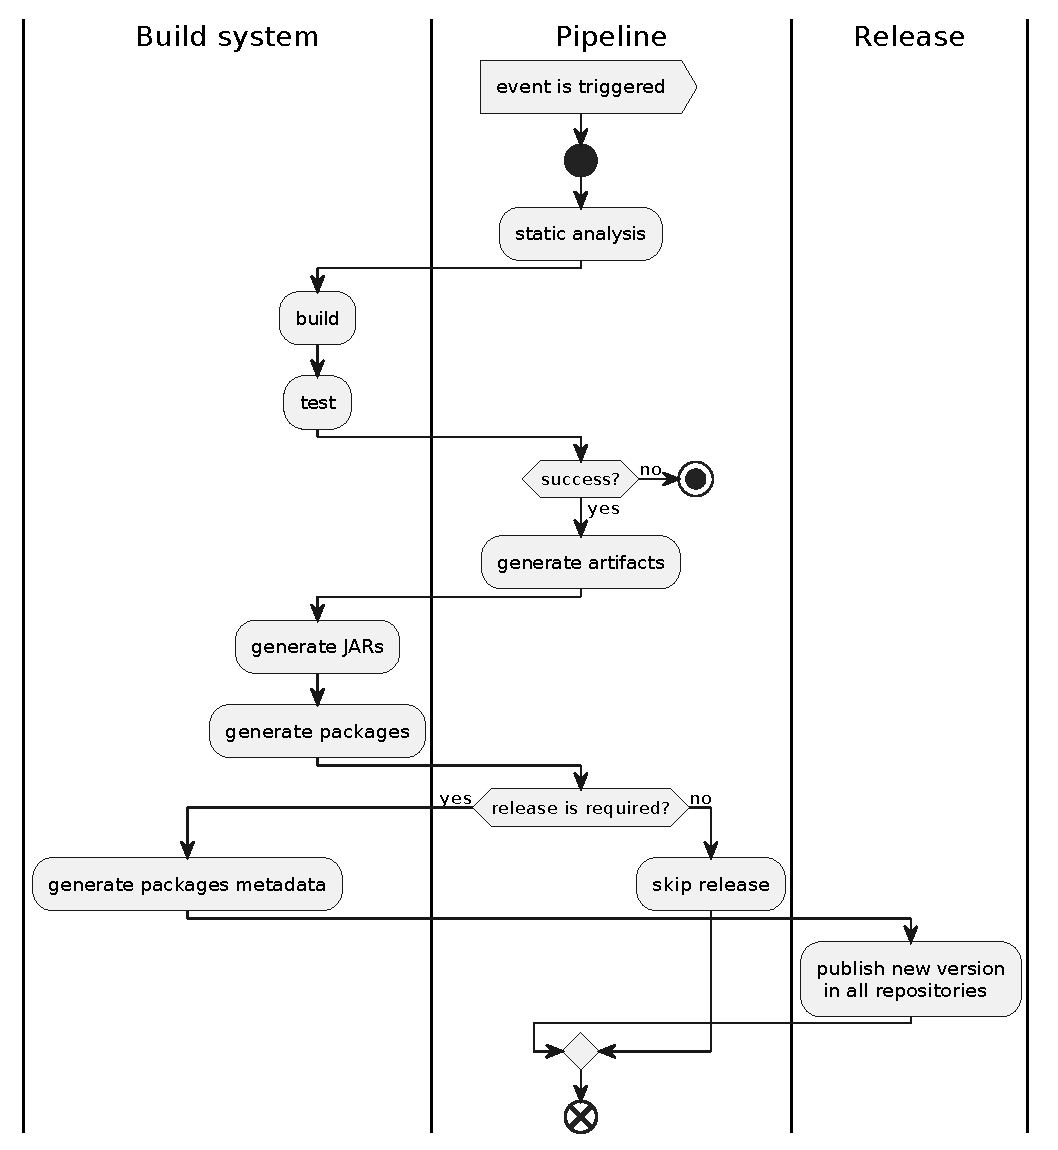
\includegraphics[width=.9\linewidth]{figures/activity-interaction-diagram.pdf}
	\caption{Diagramma delle attività raffigurante l'interazione tra i componenti}
	\label{fig:activity-interaction-diagram}
\end{figure}

Nello schema in \Cref{fig:activity-interaction-diagram} si fa riferimento ad un generico evento come segnale di avvio della pipeline. Nell'ambito \ac{cicd} l'evento corrisponde spesso alla pubblicazione di nuovo codice nel repository, in modo da generare un processo di integrazione continua del software.

\section{Configurazione del build system}

Il ruolo principale del \textit{build system} è quello di esporre un \textit{task} adibito alla generazione dei pacchetti. Il task dovrà soddisfare i seguenti requisiti:
\begin{itemize}
	\item Deve configurare correttamente le opzioni di \textit{jpackage}, in particolare quelle che mutano nel tempo come la versione.
	\item È necessario stabilire un corretto ordine di esecuzione ed albero delle dipendenze per garantire la consistenza del processo.
	\item Deve consentire la dichiarazione di configurazioni differenti a seconda del sistema operativo che esegue il processo.
\end{itemize}

\subsection{Lo strumento jpackage}\label{sec:design-jpackage}
Lo strumento \ac{cli} \textit{jpackage} offre un'interfaccia munita di diverse opzioni per configurare e personalizzare a piacimento i pacchetti in output. Esistono parametri generici, compatibili con tutte le piattaforme, e parametri specifici che vanno a modificare attributi particolari alla tipologia di pacchetto in output scelta. Uno dei motivi che ha portato alla scelta di \textit{jpackage} rispetto ad altri software è la capacità di includere autonomamente una \textit{runtime-image} di Java, ossia una \ac{jre} ridotta di dimensioni all'interno del pacchetto. La combinazione di una \textit{runtime-image} e degli archivi Java (JAR) necessari all'esecuzione dell'applicazione costituiscono l'\textit{application-image}: un pacchetto self-contained che include l'applicazione, assieme una \ac{jvm} ed alle librerie necessarie per eseguire quell'applicazione sulla piattaforma di destinazione.

\paragraph{Application image} Alchemist è un progetto modulare ed ogni modulo è distribuito in un archivio JAR specifico. Come descritto nella documentazione\footnote{https://alchemistsimulator.github.io/howtos/preparation/jar/index.html} il software predispone due modalità di utilizzo stand-alone attraverso l'esecuzione degli archivi Java. La prima modalità consiste nell'inclusione dei singoli moduli richiesti come \textit{classpath} del processo di esecuzione. La seconda modalità sfrutta l'archivio denominato ``full", ossia un \textit{fat-jar} contenente tutti i moduli e tutte le dipendenze necessarie all'esecuzione del software in tutte le sue parti. In ottica di ridurre le dimensioni del pacchetto e velocizzare il processo di impacchettamento, jpackage costruirà l'\textit{application-image} utilizzando quest'ultimo. Il risultato di un'installazione corretta è differente a seconda della piattaforma di destinazione del pacchetto, nella figura \ref{fig:application-image-folder-structure} è raffigurata l'organizzazione dei file del software installato in un sistema Linux.  

\begin{figure}
	\centering
	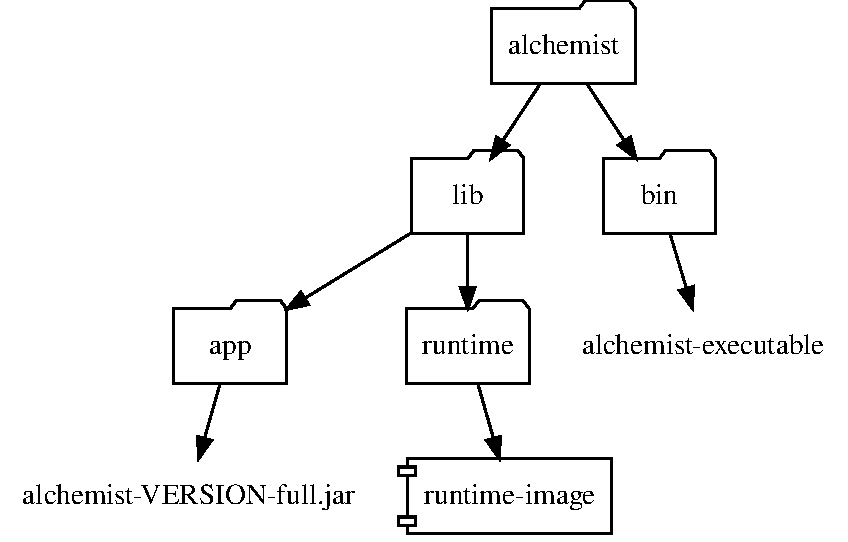
\includegraphics[width=.7\linewidth]{figures/application-image-folder-structure.pdf}
	\caption{Struttura del filesystem dell'\textit{application image} generato da \textit{jpackage} con Linux come piattaforma target}
	\label{fig:application-image-folder-structure}
\end{figure}

\paragraph{Integrazione} Per introdurre jpackage nel build system è necessario un task che funga da \textit{wrapper}: il quale esponga proprietà corrispondenti alle opzioni della \ac{cli} di jpackage. Gradle utilizza una pratica denominata \textit{lazy configuration} che fornisce la dichiarazione delle \textit{lazy properties} vale a dire ``proprietà pigre". Questa caratteristica consente di legare una proprietà ad un'altra senza doversi preoccupare dell'ordine di esecuzione. In tale modo non sono necessarie particolari attenzioni nell'assegnazione di proprietà come la versione, la quale viene calcolata da un plugin apposito. 

Il programma jpackage, come illustrato nella sezione \ref{sec:packaging}, non è \textit{cross-platform}, ciò significa che la generazione dei pacchetti deve essere eseguita su una macchina ospitante il sistema operativo di destinazione dei pacchetti richiesti. Per quanto lo strumento cerchi di unificare i diversi ambienti, ogni tipologia di pacchetto specialmente se di piattaforme diverse presenta limiti e caratteristiche differenti. Per questa ragione il task deve prevedere l'utilizzo di parametri differenti a seconda del sistema operativo sottostante.

\subsection{Design finale} Il design ultimo è raffigurato nella figura \ref{fig:gradle-jpackage-scheme}. 

\begin{figure}[htb]
	\centering
	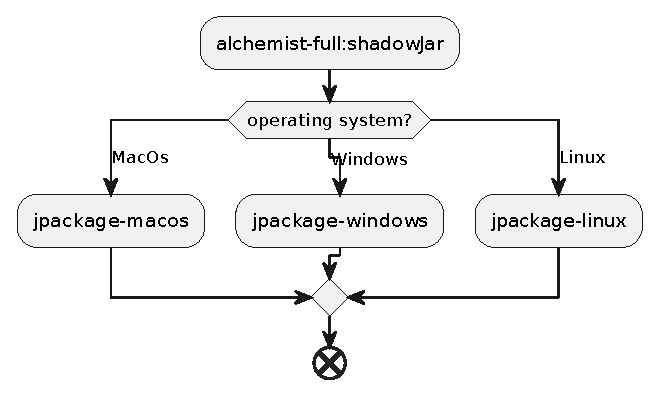
\includegraphics[width=.8\linewidth]{figures/gradle-jpackage-scheme.pdf}
	\caption{Diagramma delle attività rappresentante il processo di generazione dei pacchetti}
	\label{fig:gradle-jpackage-scheme}
\end{figure}
\noindent Come discusso nella precedente sezione il design divide la generazione nei tre sistemi operativi target e la sua esecuzione dipende da \texttt{al\-che\-mi\-st\--fu\-ll\-:sha\-dow\-Jar\-}: il task incaricato di generare l'archivio JAR full. In questo modo, quando il task incaricato di generare i pacchetti con jpackage viene invocato, in primo luogo Gradle genera l'archivio JAR necessario a jpackage per costruire un application image valido.

\section{Pipeline}
La pipeline è l'elemento chiave per generare l'automazione dei processi descritti. Alchemist è già provvisto di una pipeline, la quale si occupa di analizzare il codice, verificare i processi di rilascio e in caso sia necessario rilasciare una nuova versione. Il compito del design esplicato in questa sezione è quello di introdurre nuovi step con lo scopo di automatizzare la generazione e distribuzione dei pacchetti generati precedentemente. Le diverse unità di esecuzione o \textit{job} che popolano la pipeline possono essere distinti in base al loro ruolo.
\begin{itemize}
	\item \textbf{Inizializzazione}, tutte le unità incaricate di preparare l'ambiente di esecuzione della pipeline e quindi dei successivi job. 
	\item \textbf{Build e analisi}, i job responsabili di analizzare, compilare ed eseguire i test del codice.
	\item \textbf{Assemblaggio}, le unità di esecuzione responsabili della creazione di artefatti: archivi, pacchetti e documentazione.
	\item \textbf{Test}, job i quali verificano la validità degli artefatti o operazioni come la distribuzione.
	\item \textbf{Rilascio}, i componenti incaricati al rilascio di una nuova versione del software e le relative operazioni accessorie.
\end{itemize}
\begin{figure}[htb]
	\centering
	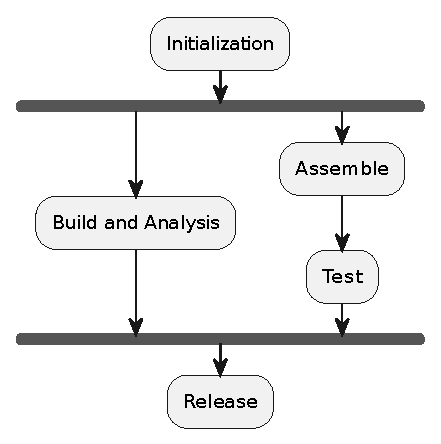
\includegraphics[width=.5\linewidth]{figures/pipeline-roles.pdf}
	\caption{Diagramma dell'attività illustrante il flusso attraverso i ruoli delineati}
	\label{fig:workflow-roles-summary}
\end{figure}
L'interazione dei processi nella pipeline è raffigurato nella \Cref{fig:workflow-roles-summary}. L'\textbf{inizializza\-zio\-ne} trova spazio al primo posto e la sua esecuzione è strettamente necessaria per il proseguimento del flusso. L'\textbf{assemblaggio} e \textbf{build} sono eseguiti parallelamente mentre i \textbf{test} devono inevitabilmente dipendere dalla fase di assemblaggio per poter verificare l'output prodotto da quest'ultimo. Il \textbf{rilascio} infine, richiede che tutte le fasi descritte precedentemente siano eseguite con successo. I ruoli concernenti il lavoro descritto da questo elaborato sono: assemblaggio, test e rilascio.

\subsection{Interazione con il Build System}

Per conseguire gli obiettivi dettati dai ruoli di assemblaggio e test è necessario l'utilizzo del build system. In particolare Alchemist sfrutta lo script \textit{gradle wrapper} per interagire con esso. Il file \textit{gradlew} è uno script che permette di eseguire Gradle senza doverlo installare globalmente: alla prima esecuzione controlla la versione richiesta definita in un file di configurazione, se quest'ultima non è presente allora il wrapper scarica questa e la utilizza per eseguire i task richiesti. I job, le unità di esecuzione della piattaforma GitHub Actions, consentono l'esecuzione di comandi nella \textit{shell} default (oppure una differente) del sistema operativo presente nel runner. In questo modo tramite comandi da shell è possibile eseguire lo script e fornire i task la cui esecuzione è richiesta come argomento di esso.

\paragraph{Test delle funzionalità} Lo \textit{status} di un job indica il risultato dell'esecuzione di esso e può essere: \textit{failure}, \textit{success} oppure \textit{skipped}. Un job è considerato in errore nel caso l'esecuzione di un comando restituisca un valore diverso da 0 e viceversa, perciò non sono necessarie particolari funzionalità per implementare un processo di verifica in quanto il comportamento comune dei comandi rispecchia le regole utilizzate. Lo stato \textit{skipped}, invece, si riferisce ai job non eseguiti secondo condizioni specifiche descritte dallo sviluppatore, è quindi possibile gestire un unico workflow e modificare il suo flusso a seconda dell'evento che ha innescato l'esecuzione. Il comportamento dei job di default all'interno di una pipeline è bloccante per cui il fallimento di uno porta all'interruzione dell'intera pipeline, come raffigurato nel diagramma \cref{fig:activity-diagram-job}.
\begin{figure}[htb]
	\centering
	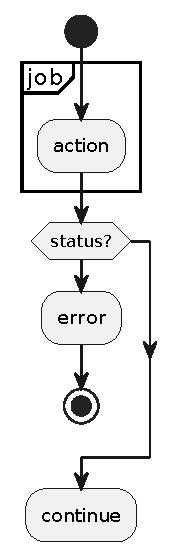
\includegraphics[width=.18\linewidth]{figures/activity-diagram-job.pdf}
	\caption{Diagramma dell'attività illustrante il comportamento dei job all'interno della pipeline}
	\label{fig:activity-diagram-job}
\end{figure}

Come raffigurato nella figura \ref{fig:pipeline-activity-diagram}, la pipeline ottenuta inserisce nuovi job adibiti all'assemblaggio ed al test dei processi. L'assemblaggio coinvolge tre unità di esecuzione operanti in runner differenti, adibiti alla pacchettizzazione del software nelle tipologie supportate. I job di test racchiudono all'interno le verifiche di validità dei pacchetti generati precedentemente e simula ove possibile la distribuzione del software.
\begin{figure}[htb]
	\centering
	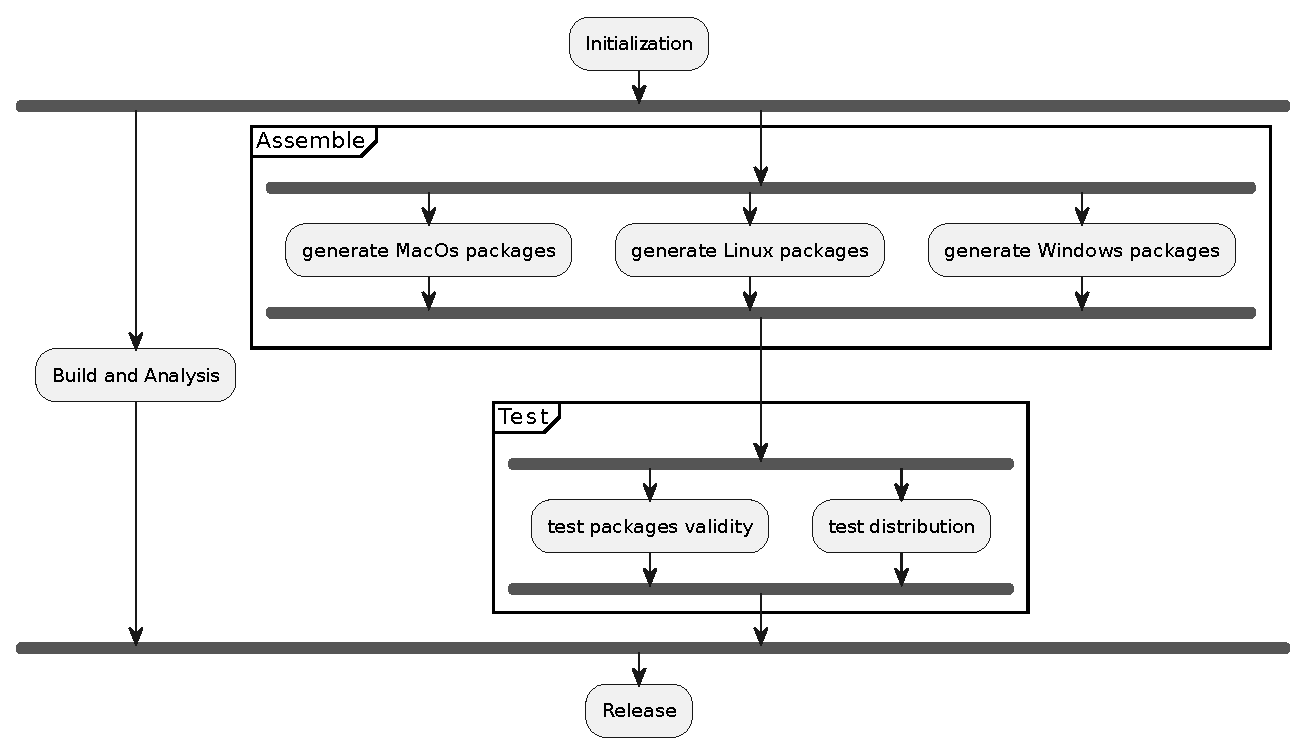
\includegraphics[width=1\linewidth]{figures/pipeline-result.pdf}
	\caption{Diagramma dell'attività della pipeline risultante}
	\label{fig:pipeline-activity-diagram}
\end{figure}

\newpage
\section{Release}

\subsection{Repository}
Nell'ambito dei package management system, i repository sono i database online da cui i gestori di pacchetti reperiscono gli applicativi. Più genericamente, si intende un qualsiasi archivio online da cui è possibile scaricare software. Ogni repository supporta tipologie di pacchetti e modalità di pubblicazione differenti, le quali sono discusse nella seguente sezione.

\paragraph{AUR} L'Arch User Repository richiede la compilazione di un file PKGBUILD, ossia uno script contenente gli step necessari a scaricare, estrarre, compilare ed infine installare il software. Lo script segue uno schema predefinito con parametri obbligatori ed altri facoltativi che modificano i meta-dati del pacchetto risultante. Oltre alla presenza di diversi attributi standard, attraverso delle funzioni predefinite è possibile modificare il processo di installazione utilizzando il linguaggio di shell scripting Bash.
Nell'ambito di questo progetto solamente la funzione \textit{package} è necessaria, in quanto il pacchetto sorgente contiene il software pronto per essere eseguito, la funzione dunque si occupa di posizionare i file nel sistema una volta che \texttt{makepkg} ha autonomamente estratto il contenuto del pacchetto di installazione. Per non modificare direttamente il filesystem del computer installante, \texttt{makepkg} crea due directory \textit{pkg} e \textit{src}. All'interno di src, esso estrae il pacchetto con tutto il suo contenuto, mentre pkg simula il filesystem del sistema. La funzione package adibita all'installazione, sposta i file dalla cartella src dentro pkg ricreando il percorso finale che si vuole ottenere sul sistema installante (considerando pkg come root). Una volta generato il pacchetto mediante makepkg, questo può essere installato utilizzando il package manager di riferimento: \textit{pacman}. Esso si occuperà di ricreare la struttura descritta all'interno della directory pkg nel filesystem del sistema installante.

I pacchetti all'interno dell'\ac{aur} consistono in repository \textit{git} contenenti il PKGBUILD ed altri file di configurazione opzionali. Il processo di pubblicazione dunque è simile a qualsiasi progetto con un sistema di version control e si articola attraverso quindi: la creazione di un commit con le modifiche al PKGBUILD e la pubblicazione di quest'ultimo.

\paragraph{Winget}\label{chap:winget} Il package manager Winget presenta una struttura simile, dove un pacchetto è composto da diversi file manifest che descrivono i metadati del pacchetto nel formato YAML. A differenza del PKGBUILD, non ci sono script e non esistono funzioni, l'intera configurazione è descrittiva e non presenta la possibilità di inserire comandi da eseguire pre o post installazione. I file manifest si distinguono in: manifesto della versione, contenente dettagli identificativi del pacchetto, il manifesto delle impostazioni locali, il quale descrive la configurazione per uno specifico locale, ed il manifesto dell'installer, contenente l'URL dove reperire il pacchetto installante ed altre informazioni specifiche. Per semplificare il processo di creazione e pubblicazione dei pacchetti, Microsoft prevede l'utilizzo di uno script ``wingetcreate" che guida l'utente nella scelta dei parametri. Questo inoltre si presta ad essere utilizzato all'interno di pipeline \ac{cicd} per aggiornare pacchetti già presenti. Il suo utilizzo è quindi necessario per assicurarsi aggiornamenti consistenti, in quanto, lo schema dei manifest può evolversi e cambiare nel tempo. Lo script si occupa autonomamente di aderire ai nuovi schemi, eliminando quindi la necessità per lo sviluppatore di aggiornare il processo di pubblicazione ogni tal volta che una nuova specifica viene pubblicata.

\subsection{Semantic release}
Il processo di \ac{cicd} utilizzato da Alchemist, prevede l'utilizzo di una tecnica chiamata \textit{semantic release}, legata con il più conosciuto concetto di \textit{semantic versioning}. Abbreviato come ``SemVer", esso è uno schema di versionamento standardizzato per determinare le versioni di un software. È stato progettato per rendere intuitivo comprendere le modifiche apportate al software ed il loro impatto riguardo la compatibilità con le versioni precedenti. Lo schema descrive una versione come tre cifre principali separate da punti.
\begin{itemize}
	\item La prima cifra, \textbf{major}, si incrementa quando vengono apportate modifiche sostanziali al software che lo rendono incompatibile con le versioni precedenti.
	\item La seconda, \textbf{minor}, indica l'aggiunta di nuove funzionalità o miglioramenti al software senza eliminare la retro-compatibilità di questo.
	\item La terza cifra, \textbf{patch}, viene incrementata quando una nuova versione risolve bug o problemi di sicurezza.
\end{itemize}
Oltre allo schema principale, SemVer prevede anche la presenza di etichette che stabiliscono se la versione è in fase di sviluppo(alpha, beta) oppure di test.
Attraverso l'utilizzo dei \textit{conventional commits}, il progetto è capace di: stabilire la versione autonomamente, elencare le modifiche tra un rilascio e quello successivo in un \textit{changelog} e decidere quando è necessaria la pubblicazione di una nuova versione. I conventional commits sono un insieme di regole che riguardano i messaggi dei commit, ossia le parti di testo allegate alla modifica del software che lo sviluppatore annette. Le regole stabiliscono una sintassi predefinita che permette di comprendere attraverso la cronologia dei commit le modifiche apportate al software, ed inoltre assieme allo schema SemVer permette a tool automatici di calcolare la versione. Nello specifico Alchemist utilizza un plugin di NodeJS capace di analizzare i commit, calcolare la nuova versione ed infine pubblicarla. Esso permette attraverso diverse estensioni di modificare il suo comportamento, in particolare: definire i file associati alla nuova versione che saranno disponibili nella release GitHub ed eseguire un comando personalizzato quando avviene la pubblicazione.

\paragraph{Limitazioni}\label{sec:release-limitation} La creazione di una release su GitHub svolta dal plugin determina il rilascio di una nuova versione del software e di conseguenza determina altresì la pubblicazione di essa nei repository pubblici. L'unica modalità per estendere il processo di rilascio e integrare la pubblicazione nei repository winget e \ac{aur} è il comando configurato attraverso il plugin. Questo dettaglio crea delle restrizioni: (i) sul sistema operativo, perché solo un job può prendere in carico il lavoro di rilascio e di conseguenza un solo runner con uno specifico sistema operativo esegue il comando e (ii) l'utilizzo inevitabile di comandi da shell. 
%!TEX root = ../thesis-main.tex

\chapter{Implementazione}

Nel seguente capitolo è illustrato il percorso e le relative scelte implementative effettuate per soddisfare i requisiti posti dal progetto. Successivamente, valuterò il lavoro svolto considerando i requisiti posti durante l'analisi.

\section{Pacchettizzazione e meta-dati}

\subsection{Pacchettizzazione}

Come discusso nelle precedenti sezioni riguardanti lo strumento jpackage (in particolare sezione \ref{sec:design-jpackage}), esso presenta una notevole quantità di opzioni sia inerenti l'aspetto estetico (nome dell'applicazione, icona, copyright e altri), sia riguardo aspetti tecnici che possono contraddistinguere la qualità del pacchetto di installazione. 

Quando si utilizza il comando jpackage per creare un pacchetto eseguibile distribuibile, è importante comprendere che questo strumento utilizza una serie di strumenti e tecnologie sottostanti per generare il pacchetto finale per diverse piattaforme. Internamente, il comando fa uso di vari strumenti di creazione di pacchetti, a seconda del sistema operativo di destinazione e del formato del pacchetto desiderato. Per esempio, su sistemi Windows, jpackage sfrutta Wix (Windows Installer XML) per creare pacchetti MSI, xCode invece è utilizzato per MacOs mentre rpm-build e fakeroot coprono rispettivamente rpm e deb. Mediante la funzionalità di \textit{override} è possibile personalizzare e modificare i file di configurazione utilizzati dai diversi strumenti in modo da controllare più a basso livello le caratteristiche dei pacchetti generati. Ciò è realizzabile sfruttando due opzioni fornite dall'interfaccia del comando stesso. Eseguendo il programma fornendo l'opzione \texttt{temp}, lo strumento inserisce all'interno della cartella designata i file temporanei, ossia i file di configurazione utilizzati internamente. In questo modo si ottiene una base su cui modificare e aggiungere funzionalità. Successivamente i file elaborati sono riposti in un percorso specifico il quale viene fornito all'opzione \texttt{resource-dir} del comando. Lo strumento durante l'esecuzione controlla il contenuto della cartella ed utilizza i file di configurazione presenti per generare i pacchetti. 

Questa funzionalità ha permesso di soddisfare il requisito \textbf{plug and play} dell'elaborato, in particolare modificando il processo di installazione e garantendo l'inserimento di Alchemist in un percorso valido per consentire l'esecuzione da riga di comando. Nello specifico, su Windows l'inserimento di un elemento \texttt{<Environment>} ha consentito di aggiungere il percorso di installazione dell'applicazione nella variabile \texttt{path} di sistema, su Linux invece i pacchetti autonomamente una volta installati, mediante l'utilizzo dei soft-link, creano un riferimento all'eseguibile posizionato nel percorso \textit{/usr/bin}, ossia la directory contenente i comandi utilizzabili dall'utente.

La capacità di sovrascrivere le configurazioni dei toolset ha permesso di ottenere un maggior controllo sulla forma e comportamento dell'installazione dei pacchetti. Le successive opzioni di carattere tecnico si occupano di modificare il contenuto di questi. In quest'ottica è necessario introdurre un altro strumento del \ac{jdk}: (i) \texttt{jlink}. Esso consente la creazione di runtime-image di java contenenti un numero minore di moduli, dunque con meno funzionalità, ma ridotte di dimensioni. Mentre un \ac{jre} globale installato su una macchina è auspicabile sia completo di tutti i suoi moduli, un ambiente privato adibito all'esecuzione di una sola applicazione beneficia di questa funzionalità riducendo lo spazio occupato dall'applicazione nel suo complesso e aumentando le prestazioni in esecuzione. 

Per costruire ambienti ad-hoc all'esecuzione di una particolare applicazione si utilizza un terzo strumento di nome \texttt{jdeps}. Quest'ultimo consente di analizzare le dipendenze di un archivio java e ottenere quindi i moduli fondamentali all'esecuzione dell'applicazione. L'utilizzo dei tre strumenti singolarmente consente di ottenere un maggior controllo sul contenuto del pacchetto, tuttavia nei casi più comuni non è necessario poiché il comando jpackage autonomamente utilizza jlink ed espone due opzioni per modificare il suo comportamento. Nel listato \ref{lst:jlink-runtime-image-creation} è descritto l'utilizzo dei tre strumenti consecutivamente per ottenere la pacchettizzazione desiderata.

\lstinputlisting[float=htb,language=Bash,label={lst:jlink-runtime-image-creation}, caption={Comandi utilizzati per generare una runtime-image ad-hoc}, captionpos=b]{listings/jpackage-jlink.sh}

\def\arraystretch{1.2}
\begin{table}[htb]
	\label{fig:jpackage-options}
	\begin{tabular}{|l|l|l|}
		\hline
		\rowcolor[HTML]{ECF4FF} 
		\multicolumn{1}{|c|}{\cellcolor[HTML]{ECF4FF}{\ul Opzione}} &
		\multicolumn{1}{|c|}{\cellcolor[HTML]{ECF4FF}{\ul Funzionalità}} &
		\multicolumn{1}{|c|}{\cellcolor[HTML]{ECF4FF}{\ul Eventuali parametri}} \\ \hline
		\texttt{--type} &
		Tipologia di pacchetto in output &
		\begin{tabular}[c]{@{}l@{}}rpm, deb, exe, msi, \\ pkg, dmg\end{tabular} \\ \hline
		\texttt{--input} &
		\begin{tabular}[c]{@{}l@{}}Directory contenente i file\\ che comporranno l'application-image \end{tabular} &
		Percorso alla directory \\ \hline
		\texttt{--main-jar} &
		\begin{tabular}[c]{@{}l@{}}L'archivio JAR principale \\ utilizzato all'avvio \end{tabular} &
		Percorso del JAR \\ \hline
		\texttt{--main-class} &
		\begin{tabular}[c]{@{}l@{}}La classe che contiene la \\ funzione di avvio\end{tabular} &
		Nome della classe \\ \hline
		\texttt{--add-modules} &
		\begin{tabular}[c]{@{}l@{}}I moduli integrati nel\\ runtime-image generato da \\ jlink\end{tabular} &
		\begin{tabular}[c]{@{}l@{}}Lista dei moduli separata\\ da ','\end{tabular} \\ \hline
		\texttt{--jlink-options} &
		\begin{tabular}[c]{@{}l@{}}Ulteriori opzioni per\\ l'esecuzione di jlink\end{tabular} &
		Lista delle opzioni \\ 
	\end{tabular}
	\caption{Tabella che elenca le principali opzioni tecniche del comando \texttt{jpackage}}
\end{table}

Il comando jdeps analizza e riporta i moduli richiesti per l'esecuzione dell'archivio fat-jar di Alchemist. Il suo output, correttamente formattato grazie all'opzione \texttt{--print-module-deps}, è diretto a jlink, il quale costruisce l'ambiente java limitato in una cartella specifica. In questa fase è possibile modificare ulteriormente la runtime-image manualmente se necessario, quest'ultima indicata come input da jpackage sarà copiata all'interno del pacchetto assieme all'archivio dell'applicazione. Gli ultimi due step possono essere riassunti in un unico comando facendo riferimento alla tabella \ref{fig:jpackage-options}:

\texttt{\\ jpackage --input build/package-input \\ \tab\tab --main-jar alchemist-full-VERSION.jar \\ \tab\tab --main-class it.unibo.alchemist.Alchemist \\ \tab\tab --add-modules \$DEPENDENCIES \\ \tab\tab --jlink-options no-header-file, no-man-pages \\}

Successive analisi hanno evidenziato come l'utilizzo di jdeps ricalca il limite citato nei capitoli precedenti, la \textit{closed world assumption}. Come per GraalVM, jdeps esegue un'analisi statica, perciò non considera l'utilizzo della reflection e di altre funzionalità dinamiche durante l'analisi delle dipendenze. Alchemist, si avvale di queste tecniche dinamiche per garantire l'estendibilità del framework, ragion per cui l'utilizzo di un ambiente \ac{jre} limitato non è consentito. Rimuovendo l'opzione \texttt{--add-modules} dal prompt, jlink adopera il comportamento di default inserendo dunque un ambiente completo.

\paragraph{Plugin} Il design elaborato nel capitolo precedente evidenziava la necessità di un task \textit{wrapper} che incapsulasse le opzioni e funzionalità di jpackage per integrare lo strumento all'interno del build system. La versatilità offerta da Gradle ha permesso di ottenere il risultato voluto attraverso \textit{jpackage-gradle-plugin}\footnote{https://github.com/petr-panteleyev/jpackage-gradle-plugin}: un plugin sviluppato dalla comunità. Questo componente introduce un tipo di task \texttt{JPackageTask} capace di: (i) configurare tutte le opzioni supportate da jpackage per qualsiasi versione del \ac{jdk}, (ii) definire blocchi di codice eseguiti solamente su un sistema operativo specifico e (iii) testare le configurazioni attraverso la modalità \textit{dry run}. Tuttavia, il plugin introdotto non risolve uno dei limiti di jpackage evidenziato in fase di analisi: la creazione di un solo pacchetto per esecuzione. Per far fronte a questa limitazione, è stata creata una tipologia personalizzata (listato \ref{lst:custom-jpackage-task}) che estende quella fornita dal plugin. In questo modo, è stato possibile modificare il comportamento del task intervenendo specificamente sul metodo contrassegnato con \texttt{@TaskAction}. Tale metodo contiene il codice eseguito quando il task viene invocato da riga di comando, avviandone l'esecuzione. 

\lstinputlisting[float=htb,language=Kotlin,label={lst:custom-jpackage-task}, caption={Definizione di un tipo di task personalizzato}, captionpos=b]{listings/custom-jpackage-task.kt}

\subsection{Meta-dati}

Nei paragrafi seguenti saranno esposte le tecniche utilizzate per garantire l'utilizzo di meta-dati conformi ai requisiti dei repository di destinazione.

\paragraph{Template} I meta-dati associati ai pacchetti presentano attributi statici e altri dinamici. Prendendo in esame il file PKGBUILD, parametri come il nome, la descrizione o le dipendenze non richiedono modifiche tra versioni differenti del software. La modifica di questi è a discrezione dello sviluppatore, il quale come manutentore si occupa per esempio di aggiornare le dipendenze manualmente o modificare le funzioni nel caso dovesse essere necessario. I parametri considerati dinamici invece, richiedono costanti modifiche perché direttamente o indirettamente sono legati alla versione per la quale si sta preparando lo script. Di seguito sono elencati i fondamentali:
\begin{itemize}
	\item la \textbf{versione}, seppure è possibile delegare il calcolo alla funzione \textit{pkgver}, quest'ultima non è ottenibile se non utilizzando il build system. Essendo necessaria l'interazione con Gradle, la scrittura di questo parametro deve essere necessariamente eseguita dinamicamente attraverso esso.
	\item la \textbf{sorgente}, ossia l'URL localizzante il pacchetto in rete. L'aggiornamento a una nuova versione richiede l'utilizzo di un nuovo pacchetto, ragion per cui l'URL sarà differente.
	\item il \textbf{checksum}, ovvero il codice hash legato alla sorgente. È utilizzato da makepkg per assicurarsi che il pacchetto installato non sia stato sostituito da un attore malevolo. Essendo legato direttamente alla sorgente, il cambiamento di questa induce un cambio del checksum.
\end{itemize}
Mediante l'utilizzo di file detti template è possibile costruire dinamicamente i meta-dati mantenendo una struttura statica facilmente aggiornabile. In particolare, il template del file PKGBUILD contiene tutti i parametri statici correttamente assegnati, mentre quelli dinamici sono identificati attraverso l'inserimento di caratteri speciali inutilizzati. Il task \texttt{generatePKGBUILD} legge il file e sostituisce i caratteri con i valori corretti ottenendo come risultato il PKGBUILD conforme e compatibile con la versione corrente del software. A differenza di Winget, il file PKGBUILD permette di utilizzare una sorgente locale (un percorso nel filesystem). Ciò è risultato particolarmente utile per verificare il funzionamento dello script in modo completo. Mediante un flag configurabile quando si invoca il task generatore si comunica a Gradle di utilizzare una sorgente locale, nello specifico il nome del pacchetto rpm. In questo modo si può simulare l'installazione del pacchetto, seppure esso non è ancora stato rilasciato all'interno dell'Arch User Repository.

\paragraph{Script} Un discorso differente vale per il repository di Microsoft dalla quale winget reperisce i pacchetti. Come citato nella sezione \ref{chap:winget}, Windows fornisce uno script interattivo capace di inserire e aggiornare nuovi pacchetti all'interno del repository. Esso permette inoltre di cercare il manifest dell'applicazione già online e aggiornarlo dallo strumento senza utilizzare file locali. Il comando necessario all'aggiornamento è così formato:

\texttt{\\wingetcreate update \$packageId --version \$packageVersion \\\tab\tab --urls "\$installerUrl" --submit --token \$gitToken}
\vspace{0.8cm}

Autonomamente lo script: (i) cerca tra i pacchetti disponibili quello indicato da \texttt{\$packageId}, (ii) aggiorna gli attributi dinamici come la versione e il pacchetto indicati dalle variabili \texttt{\$packageVersion} e \texttt{\$installerUrl}, (iii) utilizza il token GitHub per autenticarsi e richiedere attraverso una pull request l'aggiornamento del pacchetto. Mentre la modifica del pacchetto su \ac{aur} è istantanea, per winget questa deve superare un processo di validazione prima di essere eseguita con successo. Lo script, wingetcreate, in conclusione semplifica il processo e rende obsoleto l'utilizzo del build system, in quanto non è necessario comprendere il manifest del pacchetto all'interno del progetto.

\section{Sviluppo della pipeline}

L'implementazione descritta consente attraverso l'utilizzo del build system di generare i pacchetti e i corrispondenti meta-dati richiesti per la distribuzione. Il passo successivo è integrare la loro esecuzione all'interno della pipeline, in modo da conseguire gli obiettivi di integrazione e distribuzione continua. La sfida principale consiste nell'inserire i nuovi step senza stravolgere la struttura del flusso iniziale.

\subsection{Generazione degli artefatti}

Innanzitutto, il flusso richiede l'inserimento di nuovi processi incaricati di assemblare e generare gli artefatti richiesti per la distribuzione, ovvero il software impacchettato. Durante l'analisi dello strumento jpackage è stata evidenziata l'assenza del supporto al cross-platform, è necessario quindi delegare a runner con sistemi operativi differenti la generazione degli artefatti. La piattaforma Actions fornisce la possibilità di configurare una \textbf{strategia a matrice}(\cref{lst:matrix-strategy}), la quale consente di eseguire tanti job quante sono le possibili combinazioni differenti dei parametri espressi nella matrice. In questo modo descrivendo un solo job, in fase di esecuzione otteniamo diversi job paralleli i quali svolgono le stesse azioni, ma con un sistema operativo differente. Mediante l'utilizzo del build system viene richiesta la generazione dei pacchetti, e successivamente viene caricato l'output utilizzando l'azione \texttt{actions/upload-artifact}; quest'ultima permette di trasferire file al di fuori del runner, in modo che successivi job possano scaricare il loro contenuto. 

\lstinputlisting[float=htb,language=Actions,label={lst:matrix-strategy}, caption={Utilizzo della strategia a matrice per configurare job paralleli}, captionpos=b]{listings/matrix-strategy.yml}

Tramite l'attributo \texttt{if} è consentito determinare se uno step deve essere eseguito o saltato dal runner che ha preso in carico l'esecuzione, esso è risultato utile per delegare la generazione dei file JAR a solamente un sistema operativo, dato che la generazione di essi non dipende dalla piattaforma sottostante. La scelta del sistema operativo non è casuale in quanto i runner Linux sono più economici rispetto gli altri sistemi operativi forniti. Nonostante attualmente i progetti pubblici possono utilizzare l'infrastruttura di Actions gratuitamente, l'utilizzo di certe accortezze prepara il progetto a un eventuale cambio di rotta della piattaforma.

\begin{figure}[htb]
	\centering
	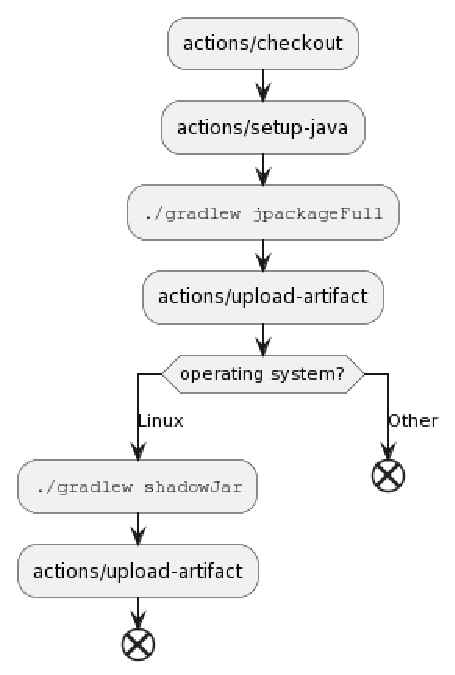
\includegraphics[width=.5\linewidth]{figures/generate-packages-job.pdf}
	\caption{Diagramma dell'attività del job incaricato a generare gli artefatti}
	\label{fig:generate-packages-job}
\end{figure}

Il job, raffigurato nella figura \ref{fig:generate-packages-job}, richiede solamente l'esecuzione di \texttt{select\--java\--version} necessaria a impostare l'ambiente java nel runner. Una volta prodotti i pacchetti, questi saranno presi in carico dai successivi job per verificare il loro corretto funzionamento.

\subsection{Il processo di rilascio}

Come esposto nella sezione \ref{sec:release-limitation}, l'aggiornamento richiesto per il rilascio del software incontra limitazioni dettate dall'impostazione della pipeline, in particolare le possibilità di sviluppo sono limitate all'utilizzo di script o comandi da shell utilizzando un runner operante Linux.

Per abilitare la pubblicazione sull'Arch User Repository, è stato introdotto uno script bash nel progetto, accessibile facilmente dal comando del plugin adibito al rilascio. Lo script gestisce l'intera operazione nei seguenti passaggi: (i) configura le impostazioni ssh necessarie per l'autenticazione e la comunicazione con il repository, (ii) clona il repository corrente e imposta le credenziali del maintainer, (iii) sostituisce il PKGBUILD con quello nuovo, e infine (iv) crea il commit e lo pubblica nel repository, completando così l'aggiornamento del pacchetto. Le informazioni richieste sono configurate come parametri e fornite direttamente nell'esecuzione; tuttavia, i valori sono privati e non devono essere accessibili al pubblico. Mediante l'utilizzo dei \textit{secrets}, GitHub consente al maintainer del progetto di configurare variabili private accessibili nella sintassi YAML di GitHub Actions utilizzando il contesto omonimo secrets. In questo modo, i valori non sono leggibili da chi visualizza il codice sorgente del progetto.

\begin{figure}[htb]
	\centering
	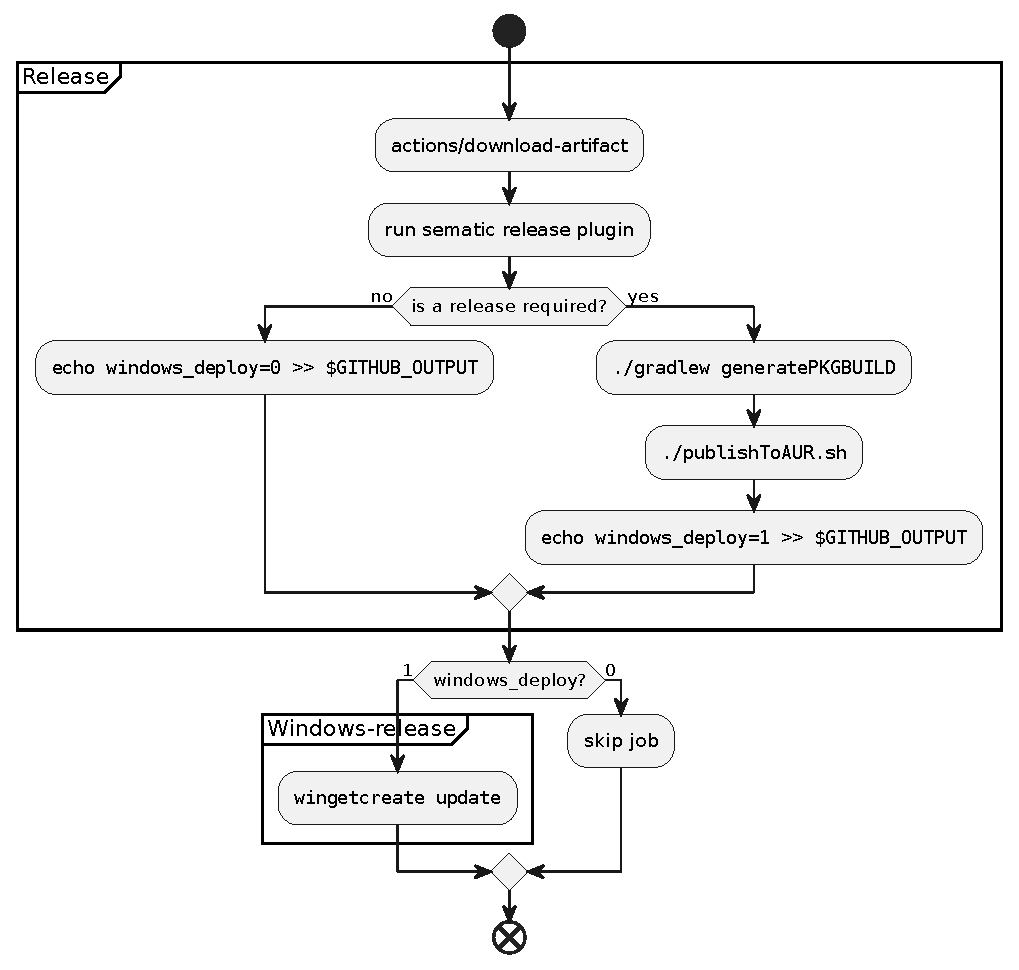
\includegraphics[width=.85\linewidth]{figures/release-flow.pdf}
	\caption{Diagramma dell'attività raffigurante il processo di rilascio su AUR e Winget}
	\label{fig:release-flow}
\end{figure}

Il processo di pubblicazione all'interno dei repository di winget richiede l'utilizzo di un runner Windows. In considerazione dei limiti e della necessità di non modificare la struttura della pipeline, è stato introdotto un job Windows complementare al rilascio. La sua esecuzione, tuttavia, deve dipendere dal plugin, il quale determina se il rilascio di una nuova versione è necessario. Nell'ottica di creare una relazione di dipendenza, il comando di pubblicazione del plugin: (i) imposta una variabile d'ambiente flag che stabilisce se il rilascio è stato eseguito, (ii) successivamente il suo valore è fornito in output mediante \texttt{\$GITHUB\_OUTPUT}, cosicché (iii) il job Windows accessorio determini se deve essere eseguito o saltato. Una rappresentazione semplificata dei due job è illustrata in una figura \ref{fig:release-flow}. Il ramo decisionale a destra descrive le azioni eseguite nel momento in cui è richiesto il rilascio di una nuova versione. La prima fase si occupa di generare il file PKGBUILD ed eseguire lo script riservato al repository AUR, mentre in un secondo momento il job complementare utilizza \texttt{wingetcreate} per procedere all'aggiornamento riguardante il package manager di Microsoft.

\subsection{Test dei processi}

Ogni processo aggiuntivo richiede lo sviluppo di un test apposito. Il fallimento di un qualsiasi test deve bloccare l'esecuzione della pipeline, cosicché si garantisce un processo di rilascio stabile e funzionante. Questa proprietà si ottiene attraverso lo sviluppo di verifiche di validità dei pacchetti e controlli riguardo la conformità dei meta-dati.

La verifica dei pacchetti richiede l'utilizzo di programmi specifici i quali dipendono dalla tipologia di pacchetto che si vuole analizzare. Utilizzando il build system e integrando un task specifico \texttt{testJpackageOutput} si collassa la definizione di molteplici job all'interno di un job unico, il quale utilizzando la strategia a matrice definita precedentemente, permette la definizione di un solo insieme di attività poi distribuito su più runner con sistemi operativi differenti. Le procedure di installazione si trovano all'interno del task, il quale conosce il sistema operativo sottostante, dunque estrae i pacchetti relativi alla sua piattaforma e controlla la presenza dei file necessari all'utilizzo dell'applicazione. Il task estende la tipologia \texttt{Exec} fornita da Gradle che permette l'esecuzione di comandi nella shell del sistema operativo, in primo luogo configura il comando adibito a installare il pacchetto a seconda della piattaforma su cui sta eseguendo (il blocco \texttt{doFirst} descritto nel listato \ref{lst:do-first-task}) e infine una volta estratti utilizza le API di Kotlin per controllare il filesystem e quindi le cartelle generate durante l'installazione (il blocco \texttt{doLast}).

\lstinputlisting[float=htb,language=Kotlin,label={lst:do-first-task}, caption={Estrazione dei pacchetti utilizzando la tipologia di task \texttt{Exec}}, captionpos=b]{listings/task-package-extraction.kt}

Inizialmente il task era posto come dipendente dall'esecuzione di jpackage, in modo che l'esecuzione del test garantisse la presenza dei pacchetti. Questo comportamento tuttavia costringe la generazione dei pacchetti ogniqualvolta si voglia eseguire la verifica. Ciò accade perché il task fornitoci dal plugin \texttt{jpackage-gradle-plugin} non dichiara alcun \textit{output}, quindi Gradle non consente di utilizzare la funzionalità della \textit{build incrementale}. In altre parole, il build system non conosce l'output del task generatore e in caso i pacchetti siano già presenti, come accade nella pipeline perché generati da job precedenti, esso riesegue la generazione sovrascrivendo gli ultimi. La rimozione della dipendenza garantisce un incremento delle prestazioni, permettendo di dividere le attività in due unità di esecuzione differenti. Il costo è una minor chiarezza nell'utilizzo manuale del task, in quanto l'esecuzione del task di verifica senza previa generazione fallirà per l'assenza dei pacchetti. Siccome il test è sviluppato principalmente per l'utilizzo all'interno di pipeline, questa limitazione non genera particolari problematiche; generalmente gli sviluppatori non eseguiranno il task sulla propria macchina, e in caso fosse necessario è sufficiente indicare l'esecuzione del task generatore assieme a quello di verifica.

\section{Valutazione e ottimizzazione}

L'implementazione descritta soddisfa i requisiti funzionali posti durante l'analisi. Lo sviluppo di nuovi processi all'interno del build system hanno consentito la pacchettizzazione del software per le piattaforme richieste mediante uno strumento esterno, jpackage. Funzionalità fornite da quest'ultimo hanno inoltre permesso una personalizzazione più approfondita dei pacchetti generati, permettendo l'esecuzione di comandi post-installazione e di conseguenza eliminando la necessità di configurazione da parte dell'utente finale. L'integrazione dei processi e delle relative verifiche all'interno della pipeline ha dato luce a un flusso di continouous delivery completo, capace di rispondere alle esigenze dettate dalla filosofia DevOps.

Lo sviluppo della pipeline ha richiesto diverse revisioni prima di ottenere il risultato finale voluto. Il flusso di integrazione e distribuzione continua per sua natura è innescato continuamente ed è perciò fondamentale sfruttare le funzionalità fornite dall'API di Actions per ottimizzare la sua esecuzione. Per ottenere l'ottimizzazione desiderata esistono diverse accortezze nella configurazione dei workflow capaci di registrare incrementi prestazionali contenuti, ma che nel lungo periodo impattano positivamente lo sviluppo del progetto. Le principali ottimizzazioni utilizzate sono elencate di seguito:
\begin{itemize}
	\item \textbf{Fail-fast}: questa ottimizzazione si applica ai flussi di lavoro che definiscono una strategia a matrice. Se il fail-fast è abilitato, la piattaforma annullerà tutti i compiti in corso e in coda nella matrice non appena uno qualsiasi dei compiti in essa fallisce.
	\item \textbf{Concurrency group}: consente di inserire job all'interno di gruppi, identificati da una chiave, nella quale un solo job per volta viene eseguito. Normalmente Actions permette l'esecuzione dello stesso workflow, job e step parallelamente, ciò significa che la pubblicazione di diversi commit rapidamente innesca l'esecuzione di più flussi paralleli. Se il flag \texttt{cancel-in-progress} è attivo e durante l'esecuzione di un job un altro componente dello stesso gruppo viene inserito in coda, quest'ultimo prende il posto ed elimina il job corrente.
	\item \textbf{Artefatti}: l'utilizzo delle action \textit{upload-artifact} e \textit{download-artifact} consentono di distribuire gli artefatti tra i job dei workflow. In generale, l'approccio preferibile è di stabilire dei job assemblatori che generano e forniscono gli artefatti a successivi job di test o rilascio. Il caricamento di file anche di notevoli dimensioni è estremamente più conveniente rispetto alla rigenerazione; file di dimensioni dell'ordine delle centinaia di megabyte sono processati in poche decine di secondi.
	\item \textbf{Timeout}: invece di fare affidamento sul timeout predefinito dei compiti, che è di 360 minuti (6 ore), i flussi di lavoro possono impostare esplicitamente un timeout personalizzato. L'opzione risulta efficace per interrompere i flussi di lavoro che si protraggono inutilmente a lungo, il che può essere particolarmente utile per evitare che i contributori, tramite pull request, inneschino flussi di lavoro prolungati.
	\item \textbf{Build system}: esso, nel caso specifico di Gradle, introduce un overhead dettato dalla necessità a ogni esecuzione di effettuare le fasi di inizializzazione e configurazione. Sebbene implementi tecniche di ottimizzazione, l'utilizzo di Gradle, in particolare nei progetti di grandi dimensioni, può incrementare il tempo di esecuzione di un job di diversi minuti.
\end{itemize}

Si propone dunque un'analisi di quattro differenti versioni di pipeline sviluppate per Alchemist. La prima (\textit{a}) rappresenta il processo di integrazione e distribuzione continua utilizzato prima dell'intervento del progetto descritto in questo elaborato. Ciò ci consente di misurare il risultato ottenuto con le successive versioni in relazione al requisito non funzionale prestazionale introdotto in fase di analisi. La seconda (\textit{b}) descrive una struttura a job paralleli, la quale utilizza il build system sia per generare che per testare gli artefatti. La terza (\textit{c}) versione utilizza una configurazione sequenziale con distribuzione degli artefatti mediante le azioni di \texttt{upload/download-artifact}, mentre la quarta (\textit{d}), e ultima versione, utilizza una configurazione prevalentemente sequenziale con caricamento degli artefatti, ma privata dell'utilizzo del build system nei job adibiti ai test. I tempi presi in esame sono ottenuti mediante la media aritmetica di dieci differenti esecuzioni dei flussi: l'\textit{execution time} indica il tempo di esecuzione del flusso nel suo complesso, mentre la \textit{total execution time} fa riferimento alla somma dei tempi di esecuzione di tutti i job all'interno della pipeline. Le quattro istanze prese in esame coinvolgono il normale flusso di integrazione e quindi non integrano l'esecuzione del job di rilascio.

\begin{figure}[htb]
	\centering
	\begin{tikzpicture}
		\begin{axis}[
			ybar,
            width=12cm,
			height=8cm,
			bar width=15,
			ylabel={ Time (h) },
			symbolic x coords={a, b, c, d},
			xtick=data,
			xlabel={Version},
			legend style={at={(0.5,-0.2)},
				anchor=north,legend columns=-1},
			]
			
			\addplot[blue!50!cyan,fill=blue!50!cyan] coordinates {(a, 0.81) (b, 0.77) (c, 1.12) (d, 0.74)};
			\addplot[red!70!orange,fill=red!70!orange] coordinates {(a, 2.12) (b, 2.55) (c, 3.11) (d, 2.78)};
			
            % Draw horizontal lines
			\legend{Execution Time, Total Execution Time}
		\end{axis}
	\end{tikzpicture}
	\caption{Grafico illustrante i tempi di esecuzione delle quattro differenti versioni di pipeline implementate}
	\label{fig:histogram}
\end{figure}
 
Innanzitutto, i risultati confermano un ottimo riscontro in relazione al requisito non funzionale, in particolare le due versioni \textit{b} e \textit{d} offrono prestazioni comparabili e contemporaneamente funzionalità aggiuntive rispetto la prima versione. L'utilizzo del build system peggiora le prestazioni, in quanto la quarta versione privata del suo utilizzo offre un miglioramento sostanziale rispetto la terza, la quale utilizza una configurazione similarmente sequenziale. La seconda versione (\textit{b}) ottiene risultati comparabili alla quarta (\textit{d}), nonostante non utilizzi il caricamento e scaricamento degli artefatti. Questo è dovuto alla mancanza del job incaricato al rilascio all'interno dei flussi analizzati. Mentre la versione \textit{d} ottiene gli artefatti da job assemblatori eseguiti precedentemente, la versione \textit{b} li genera nuovamente prima del loro rilascio. Di conseguenza, lo stesso test condotto su esecuzioni del flusso completo avrebbe mostrato un netto vantaggio della quarta versione rispetto alle altre prese in considerazione.

Dall'analisi dei dati risulta evidente come l'interazione con il build system, in particolare Gradle, prolunga l'esecuzione dei task per via delle fasi di inizializzazione dello strumento. L'utilizzo di un task, \texttt{testJpackageOutput}, per verificare la validità dei pacchetti, è risultato quindi controproducente. Sebbene quest'ultimo permetta una configurazione semplificata nel workflow, l'utilizzo di comandi shell è maggiormente indicato per svolgere semplici azioni che non richiedono particolari dipendenze.
%!TEX root = ../thesis-main.tex

\chapter{Conclusioni}
Quanto discusso nell'elaborato ha consentito la distribuzione automatica del software Alchemist nei formati standard delle piattaforme coinvolte, che rappresentano due famiglie di sistemi operativi completamente differenti. Gli obiettivi posti sono stati raggiunti grazie a una valutazione degli strumenti adibiti alla pacchettizzazione che il panorama \ac{jvm} offre, e grazie all'utilizzo di tecnologie come Gradle e GitHub Actions, sono state integrate all'interno del flusso di integrazione e distribuzione continua del progetto. L'autovalutazione ha poi evidenziato l'ottimo risultato ottenuto rispetto l'iniziale flusso di integrazione utilizzato dal software prima dell'intervento di questo progetto.

\begin{figure}[htb]
	\centering
	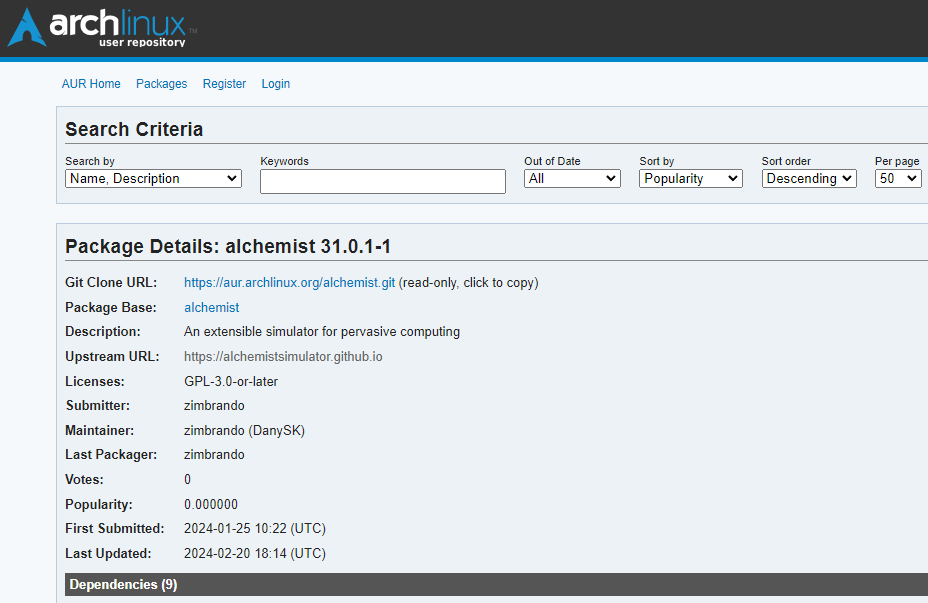
\includegraphics[width=.8\linewidth]{figures/alchemist-aur.png}
	\caption{Pagina web raffigurante il pacchetto Alchemist pubblicato sul repository AUR}
	\label{fig:aur-web}
\end{figure}

Il conseguimento degli obiettivi è osservabile su GitHub nella sezione dei rilasci\footnote{https://github.com/AlchemistSimulator/Alchemist/releases}, dove è possibile notare la possibilità di scaricare i diversi pacchetti installanti per ogni sistema operativo. Mediante invece l'utilizzo dei package manager è possibile installare ed aggiornare Alchemist con l'utilizzo di un semplice comando. Su Windows, previa installazione di winget, attraverso:
\texttt{winget install Unibo.alchemist}
e su Arch e derivate, previa autorizzazione all'installazione dall'Arch User Repository\footnote{https://aur.archlinux.org/packages/alchemist}(\Cref{fig:aur-web}), tramite \texttt{pamac} per Manjaro o più generalmente \texttt{yay}.
L'utilizzo dei package manager assicura all'utente l'installazione dell'ultima versione di Alchemist e mediante le funzionalità da questo offerte è altrettanto semplice aggiornare la sua versione, in modo da garantire l'utilizzo agli utenti delle ultime funzionalità del simulatore. 

\section{Sviluppi futuri}
L'implementazione descritta da questo elaborato ha aperto nuove possibilità di distribuzione del progetto mediante l'introduzione della pacchettizzazione. Attraverso lo sviluppo di processi automatici di pubblicazione il software è stato distribuito all'interno di due principali repository di riferimento. Le possibilità di estensione del progetto sono numerose, in quanto esistono molteplici package manager nel panorama esteso dei sistemi operativi. Nei seguenti punti sono riassunti i principali spunti per migliorare ed estendere il processo:
\begin{itemize}
	\item \textbf{Distribuzione su Homebrew}: i repository su cui Alchemist è distribuito non comprendono il sistema operativo MacOs. Il package manager Homebrew realizzato per MacOs rappresenta una valida opzione per raggiungere un pubblico più ampio attraverso modalità di installazione semplici e funzionali.
	\item \textbf{Supporto a Snap}: un'altra tipologia, nell'ambiente Linux, sono i pacchetti detti containerizzati, ovvero eseguiti all'interno di ambienti separati con un accesso limitato al sistema. Questa caratteristica fornisce due principali vantaggi: la possibilità per una applicazione di usare la propria versione desiderata di librerie di sistema senza creare conflitti e la trasparenza all'utente nell'accesso alle risorse di sistema, garantendo quindi un livello aggiuntivo di sicurezza. È il caso dei pacchetti \textit{snap}, pacchetti self-contained considerati universali perché compatibili con una notevole quantità di distribuzioni Linux. La loro implementazione nel flusso di integrazione e distribuzione continua di Alchemist contribuirebbe a un ulteriore ampliamento delle distribuzioni supportate dal software. 
\end{itemize}


%----------------------------------------------------------------------------------------
% BIBLIOGRAPHY
%----------------------------------------------------------------------------------------

\backmatter

\nocite{*} % comment this to only show the referenced entries from the .bib file

\bibliographystyle{alpha}
\bibliography{bibliography}

\end{document}